%%%%%%%%%%%%%%%%%%%%%%%%%%%%%%%%%%%%%%%%%
% Report about achieving the Java Apprentice Badge
% Using template:
% Stylish Article
% LaTeX Template
% Version 2.0 (13/4/14)
%
% This template has been downloaded from:
% http://www.LaTeXTemplates.com
%
% Original author:
% Mathias Legrand (legrand.mathias@gmail.com)
%
% License:
% CC BY-NC-SA 3.0 (http://creativecommons.org/licenses/by-nc-sa/3.0/)
%
%%%%%%%%%%%%%%%%%%%%%%%%%%%%%%%%%%%%%%%%%

%----------------------------------------------------------------------------------------
%	PACKAGES AND OTHER DOCUMENT CONFIGURATIONS
%----------------------------------------------------------------------------------------

% create labels for figures, listings and tables
% TODO: format all Java keywords with \lstinline[columns=fixed]{put keyword here}
% TODO: Format and clean up code
% TODO: make sure all classnames are in proper case in the text
% TODO: make sure the code is the latest
% TODO: refer to the line numbers in the code, when explkaining it

\documentclass[twoside,fleqn,10pt]{SelfArx} % Document font size and equations flushed left
\usepackage{listings}
\usepackage[utf8]{inputenc}
\usepackage[T1]{fontenc}
\usepackage{tabulary}
\usepackage{lipsum} % Required to insert dummy text. To be removed otherwise
\usepackage[toc,page]{appendix}
\usepackage{float}
\usepackage{wrapfig}
\usepackage{pgfplots}
\usepackage[export]{adjustbox}
\usepackage{framed}
\usepgfplotslibrary{patchplots}
\usetikzlibrary{pgfplots.groupplots}
\pgfplotsset{compat=1.12} 
 \usepackage{pifont}
 \usepackage{adjustbox}
\usepackage{array}
\usepackage{booktabs}
\newcolumntype{R}[2]{%
    >{\adjustbox{angle=#1,lap=\width-(#2)}\bgroup}%
    l%
    <{\egroup}%
}
\newcommand*\rot{\multicolumn{1}{R{90}{1em}}}% no optional argument here, please!

%----------------------------------------------------------------------------------------
%	COLUMNS
%----------------------------------------------------------------------------------------

\setlength{\columnsep}{0.55cm} % Distance between the two columns of text
\setlength{\fboxrule}{0.75pt} % Width of the border around the abstract

%----------------------------------------------------------------------------------------
%	COLORS
%----------------------------------------------------------------------------------------

\definecolor{color1}{RGB}{0,0,90} % Color of the article title and sections
\definecolor{color2}{RGB}{0,20,20} % Color of the boxes behind the abstract and headings

\definecolor{mygreen}{rgb}{0,0.6,0}
\definecolor{mygray}{rgb}{0.5,0.5,0.5}
\definecolor{mymauve}{rgb}{0.58,0,0.82}
\definecolor{lightgray}{rgb}{0.95,0.95,0.95}
\usepackage{qrcode}	
%----------------
% LISTINGS
%----------------

\lstset{ %
  prebreak=\raisebox{0ex}[0ex][0ex]
        {\ensuremath{\hookleftarrow}},
  backgroundcolor=\color{lightgray},   % choose the background color; you must add \usepackage{color} or \usepackage{xcolor}
  basicstyle=\footnotesize,        % the size of the fonts that are used for the code
  breakatwhitespace=false,         % sets if automatic breaks should only happen at whitespace
  breaklines=true,                 % sets automatic line breaking
  captionpos=b,                    % sets the caption-position to bottom
  commentstyle=\color{mygreen},    % comment style
  deletekeywords={...},            % if you want to delete keywords from the given language
  escapeinside={\%*}{*)},          % if you want to add LaTeX within your code
  extendedchars=true,              % lets you use non-ASCII characters; for 8-bits encodings only, does not work with UTF-8
  frame=single,                    % adds a frame around the code
  keepspaces=true,                 % keeps spaces in text, useful for keeping indentation of code (possibly needs columns=flexible)
  keywordstyle=\color{blue},       % keyword style
  morekeywords={*,...},            % if you want to add more keywords to the set
  numbers=left,                    % where to put the line-numbers; possible values are (none, left, right)
  numbersep=5pt,                   % how far the line-numbers are from the code
  numberstyle=\tiny\color{mygray}, % the style that is used for the line-numbers
  rulecolor=\color{black},         % if not set, the frame-color may be changed on line-breaks within not-black text (e.g. comments (green here))
  showspaces=false,                % show spaces everywhere adding particular underscores; it overrides 'showstringspaces'
  showstringspaces=false,          % underline spaces within strings only
  showtabs=false,                  % show tabs within strings adding particular underscores
  stepnumber=2,                    % the step between two line-numbers. If it's 1, each line will be numbered
  stringstyle=\color{mymauve},     % string literal style
  tabsize=2,                       % sets default tabsize to 2 spaces
  title=\lstname,                   % show the filename of files included with \lstinputlisting; also try caption instead of title
  belowskip=-\baselineskip         % no empty line after
}

\usepackage{adjustbox}
%----------------------------------------------------------------------------------------
%	HYPERLINKS
%----------------------------------------------------------------------------------------

\usepackage{hyperref} % Required for hyperlinks
\hypersetup{hidelinks,colorlinks,breaklinks=true,urlcolor=color2,citecolor=color1,linkcolor=color1,bookmarksopen=false,pdftitle={Title},pdfauthor={Author}}

%----------------------------------------------------------------------------------------
%	ARTICLE INFORMATION
%----------------------------------------------------------------------------------------

\JournalInfo{Professional Development Program Series, Vol. I, No. 1, 1-5, 2014} % Journal information
\Archive{\copyright{} Copyright Marko Viitanen, 2014} % Additional notes (e.g. copyright, DOI, review/research article)

\PaperTitle{Java Apprentice Badge Report} % Article title

\Authors{Marko Viitanen\textsuperscript{1}*} % Authors
\affiliation{\textsuperscript{1}\textit{FamilySearch, Salt Lake City}} % Author affiliation

\Keywords{Java --- Professional Development Program --- Badges} % Keywords - if you don't want any simply remove all the text between the curly brackets
\newcommand{\keywordname}{Keywords} % Defines the keywords heading name

%----------------------------------------------------------------------------------------
%	ABSTRACT
%----------------------------------------------------------------------------------------

\Abstract{As part of the professional development program we are provided a way to learn and demonstrate our development skills by earning badges. There are several badges, Java being one of them. This document describes learnings and answers to the requirements for earning the Apprentice Java Badge.}

%----------------------------------------------------------------------------------------

\begin{document}

\flushbottom % Makes all text pages the same height

\maketitle % Print the title and abstract box

\tableofcontents % Print the contents section

\thispagestyle{empty} % Removes page numbering from the first page

%----------------------------------------------------------------------------------------
%	ARTICLE CONTENTS
%----------------------------------------------------------------------------------------

\section*{Introduction} % The \section*{} command stops section numbering

\addcontentsline{toc}{section}{Introduction} % Adds this section to the table of contents

The Java Apprentice Badge is the first badge in the Java series. It covers intermediate concepts of Java programming. It is not a 101 course in programming, so many of the common language features are not covered. The requirements don't include installation, 

High-level requirements\footnote{See confluence for full description of the requirements at \url{https://almtools.ldschurch.org/fhconfluence/display/Product/Core+Skills+-+Java+-+Apprentice} .} include:
\begin{itemize}
\item Object life cycle
\item Exceptions
\item Polymorphism
\item Collections
\item Using a library
\end{itemize}

Each apprentice is allowed to creatively demonstrate their knowledge on the required topics. I chose to write a report about it.
\section{Core Java}

The first section deals with Java primitives, objects and their life cycle, and some JDK-provided classes for String manipulation and Collections. It includes writing applications to sort Strings. It also deals with Exceptions and Enums.

\subsection{Object Life cycle}
\begin{center}\textit{Describe the life cycle of an object instance in Java and how garbage collection works}\end{center}

\subsubsection{Procedural Programming} 
Procedural programming preceded object-oriented programming. Basically, The code was written line by line, like a recipe. The computer would execute the lines in the order they appeared in the program. There were constructs to jump from one place to another, called gotos. But very quickly a program can become quite complicated, and specially the gotos would make it very hard to follow. 

With many lines of code, the program becames difficult to maintain. We can split the program into several files and import the pieces when compiling. That helps humans to organize the data but also fulfills the need for the compiler to have all the pieces of the program available. It doesn't solve the problem of scope, though. In procedural programming the data is accessible to the entire program. There is no clear ownership of data.

Procedural programming also provided constructs called subroutines. They are blocks of code, collections of instructions. Subroutines have their own scope, but any data they need to access outside the subroutine is still exposed to the entire program.

\begin{figure*}[!htp]\centering % Using \begin{figure*} makes the figure take up the entire width of the page
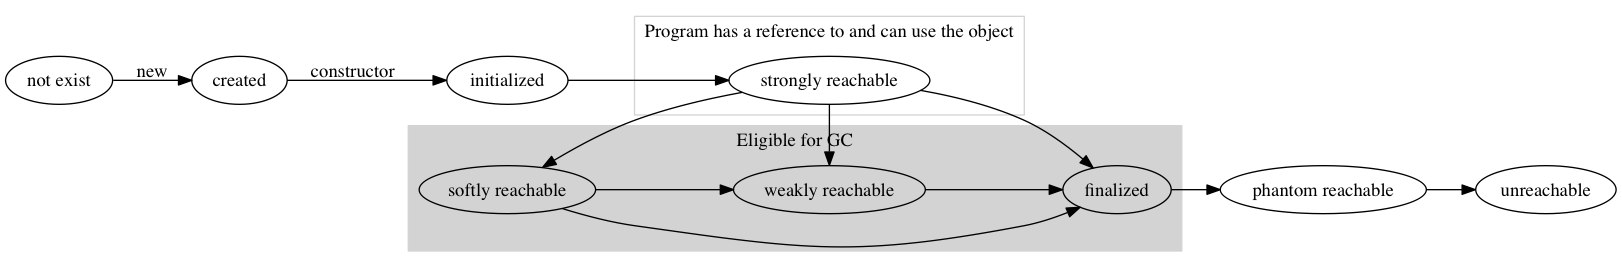
\includegraphics[width=\textwidth]{object-life-cycle.png}
\caption{Object Life Cycle}
\label{fig:object-life-cycle}
\end{figure*}

\subsubsection{Java is an Object-Oriented Language.} In object-oriented languages, instead of having data and subroutines, we deal with objects that have data and behavior. WIth object-oriented programming we can easily model the real world. For example we can have an object of a dog that has data (color, breed) and behavior (barks, runs, drools). 

When developers write java programs, they write classes. A class is like a blueprint of an object, it defines the object. A class becomes an object when we instanciate it, we create an instance of it. Obects live when the program is executing, at runtime.

With objects it is easy to encapsulate behavior and data. We can restrict access to the data to only the members inside of a class. Nobody outside the class can access the data, if we don't want to ( and we shouldn't want to.) We can define interfaces that provide indirect, controlled access to the data inside the class.

Organizing code becomes easier too, because each file can only have one  public class per file. Since each class encapsulate one "thing", that has a well-defined interface that determines its behaviors, the code becomes very logical.

Everything in Java is made of another object. We call this inheritance. Java provides the mother of all objects, called \texttt{Object}, from which any other class must inherit.

\subsubsection{Instantiating a class}
We create an object from a class with the Java keyword \texttt{new}. Before instantiation, the object doesn't exist. After instantiation it exists. Classes have a special method called a constructor. After creating the class the Java Virtual machine (JVM) calls the object's constructor. If you don't provide a constructor for your class, the its parent (eventually the \texttt{Object} constructor is called. The constructor is a place where you could initialize the object or start resources.\cite{nicholas}
\begin{figure}[H]\centering % Using \begin{figure*} makes the figure take up the entire width of the page
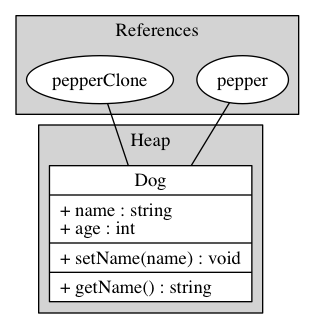
\includegraphics[width=0.5\linewidth]{object-reference}
\caption{Object References}
\label{fig:object-references}
\end{figure}
\subsubsection{Strongly Referenced}
When the constructor has been called, your program has a strong reference to it.\cite{reference} It means you can access the non-private methods and data on it. It is usable by your program.
\begin{lstlisting}[language=Java]
Dog pepper = new Dog();
\end{lstlisting}
In the above example, \texttt{pepper} is the handle to your object, or a reference. It is a strong reference (as opposed to a weak reference) because you can use it to do things with the \texttt{pepper} object:
\begin{lstlisting}[language=Java]
pepper.bark();
\end{lstlisting}

You can have several references to the same object:
\begin{lstlisting}[language=Java]
// create an instance of Dog
Dog pepper = new Dog();

// pepperClone also points to the same object
pepperClone = pepper;

// set pepper's name to "pepper"
pepper.setName("pepper");

// returns "pepper"
pepperClone.getName();

\end{lstlisting}
(See source on page \pageref{App:AppendixA}.)
In the above example we created an instance of a \texttt{Dog} and got back a reference to it called \texttt{pepper}. Then we made \texttt{pepperClone} also point to the same object. After that we set the name of \texttt{pepper} to "pepper". Because \texttt{pepper} and \texttt{pepperClone} point to the exact same object, when we ask \texttt{pepperClone} for its name, we get "pepper".

\subsubsection{Other references}
Once you let go of all the references to an object, it becomes eligible for garbage collection. The JVM still holds a weak or soft reference to the object (so it can manage it), but eventually, when it detects that memory needs to be cleaned up, it will finalize the object.\cite{reference}
\begin{figure}[H]\centering % Using \begin{figure*} makes the figure take up the entire width of the page
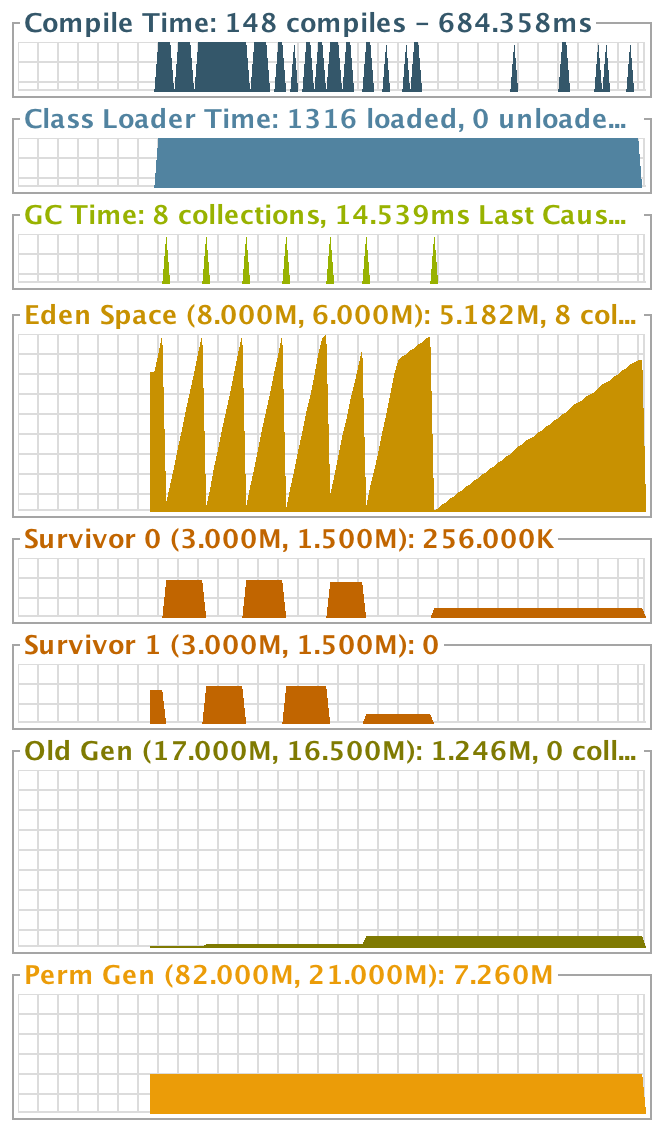
\includegraphics[width=\linewidth]{garbage-collection}
\caption{Garbage Collection}
\label{fig:garbage-collection}
\end{figure}
\subsubsection{Garbage Collection.}
When the JVM determines that it needs to free memory, it will perform a garbage collection. The soft and weak references will be cleared before throwing an \texttt{OutOfMemoryException}. 

Garbage collection is controlled by the JVM. There are tweaks you can do to suggest a certain behavior to the garbage collector, and you can even suggest that it will do garbage collection (generally not a good idea), but eventually the garbage collector will decide when to run.

The benefit of garbage colection is that the programmer doesn't need to think about finalizing objects. When they are not needed, they may be thrown into garbage automatically. There are times when this thinking can get you into troublem though. If you don't release the references the objects will never be garbage collected. An object is released when the program no longer holds a reference to it. You can either set the reference to null or it will automatically be released when your object goes out of scope.

Figure \ref{fig:garbage-collection} shows garbage collection in action. I wrote a little program that creates objects and puts them in a collection. I used the visualvm tool provided in the Oracle JDK distribution\cite{garbagecollection}. After every 10000 objects I clear the collection. I wrote created a total of 306,480,000 objects, so I cleared the collection over 30,000 times. Garbage collection, though only kicked in 7 times. I had set my heap size to 25MB. 

In the image you can also see the movement of objects from one generation to another.

\subsection{Basic Data Types}
\textit{Describe how the basic data types are represented in memory (boolean, int, long, String, array of ints, array of Objects, class with fields)}
\subsubsection{Java's Primitive Types} 
Java's primitive types can be divided into two\footnote{Really, there are three. The third one, \texttt{returnAddress}, is not available for the programmer} main groups: numeric primitives, and boolean. Numeric primitives consist of integral and floating point primitives.\cite{gosling}

\begin{figure}[H]\centering
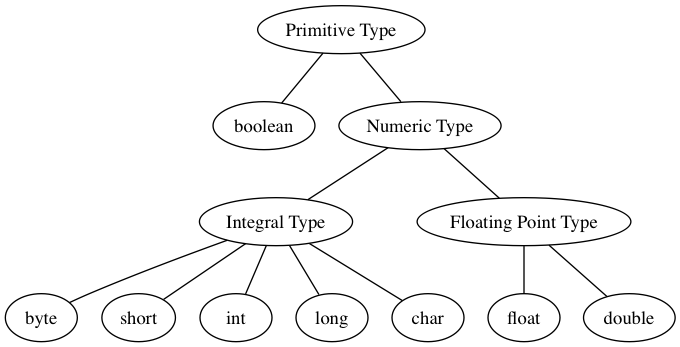
\includegraphics[width=\linewidth]{primitives.png}
\caption{Primitive Classification}
\label{fig:results}
\end{figure}

Java specification\cite{gosling} defines sizes and ranges for primitive types. The integer types are clear cut, but the floating point types are not so simple. They follow the ANSI/IEEE Standard 754-1985\footnote{see http://docs.oracle.com/javase/specs/jls/se7/html/jls-4.html\#jls-4.2.3 for details}. The values in table~\ref{tab:java-primitive-types} are from my MacBookPro, printing out the max value for float and double. They might be different on a different architecture.

Also to note that although Java defines the primitive sizes, on different architectures might actually use different sizes. For example, although an int is defined as 32 bits, it might take 64 bits on a 64 bit computer. The primitive sizes defined in the Java Specification is how the programmer sees the types, not necessarily how they are stored.

The list of primitives in Java\cite{gosling}:
\begin{table}[!htb]
\centering
\begin{tabulary}{\columnwidth}{ |>{\raggedright\arraybackslash} p{0.15\columnwidth} | >{\raggedright\arraybackslash}p{0.1\columnwidth} | >{\raggedright\arraybackslash}p{0.59\columnwidth} |}
\hline
\textbf{Type} & \textbf{Size (bits)} & \textbf{Range} \\ \hline 
byte  & 8  & from -128 to 127, inclusive \\ \hline 
short & 16 & from -32768 to 32767, inclusive \\ \hline 
int   & 32 & from -2147483648 to 2147483647, inclusive \\ \hline 
long  & 64 & from -9223372036854775808 to 9223372036854775807, inclusive \\ \hline
char  & 16 & from '\textbackslash{}u0000' to '\textbackslash{}uffff' inclusive, that is, from 0 to 65535 \\ \hline 
float & 32 & from -3.4028235E38 to 3.4028235E38\footnotemark[3] \\ \hline
double & 64 &from -1.7976931348623157E308 to 1.7976931348623157E308\footnotemark[3] \\ \hline
boolean & 32\footnotemark[4] & true or false \\ \hline
\end{tabulary}
\caption{Java Primitive Types}\label{tab:java-primitive-types}
\end{table}

\footnotetext[3]{Java float and double follow the  ANSI/IEEE Standard 754-1985, see http://docs.oracle.com/javase/specs/jls/se7/html/jls-4.html\#jls-4.2.3}
\footnotetext[4]{\texttt{boolean} is internally implemented like an \texttt{int}}
\subsubsection{Heap and Stack}
Java virtual machine memory is divided into two types; stack and the heap. Each thread gets its own stack. The heap is shared. The stack is divided into frames, which contain slots for data, called local variables, and other things. There is one frame per method call.

The JVM Specification doesn't actually specify where the different data types are stored. It specifies that the stack can store data that is needed. The frames in the stack can be heap allocated.

Usually, though, in the past the stack is used for storing primitive data, addresses to the heap, and return data. The heap holds more complex information, such as objects and arrays. A good rule of thumb is that if you create something using the keyword "new" it will end up in the heap.

Primitives are stored in the stack. Types boolean, byte, char, short, int, and float occupy one "local variable" slot in the stack frame. Types long or double occupy two slots. \cite{gosling}
\begin{figure}[H]\centering
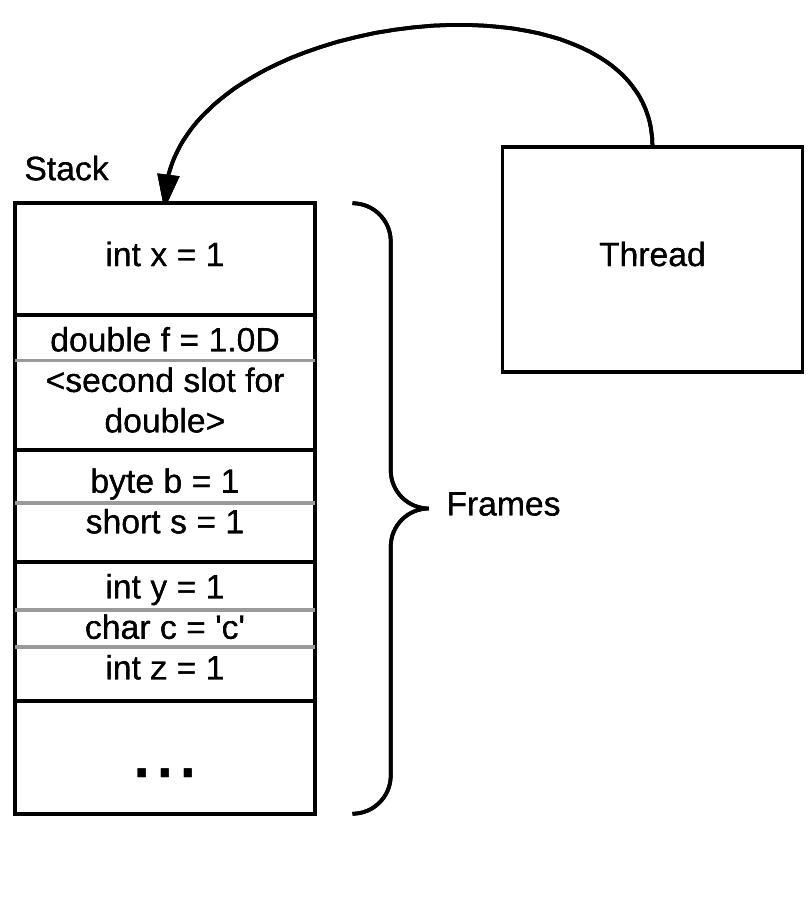
\includegraphics[width=0.9\linewidth]{images/stack}
\caption{The Stack}
\label{fig:stack}
\end{figure}
Figure \ref{fig:stack} depicts a thread with a stack that has four frames in it. The first frame has one primitive stored in it (an integer). The second one has one double, that takes up two "local variable" slots. The third and fourth frame have two and three primitives, respectively.

\subsubsection{Class With Fields on the Heap}
The stack is for simple data, like the primitives. They take up a predefined space of space. Objects are variable in size. Even two objects, created from the same class can be different in size. Objects cannot be stored in the stack, they are stored in the heap.

The reference to the object is stored in the stack. The reference points to an address in the heap, which contains the class and its fields.\cite{gosling}
\begin{figure}[H]\centering
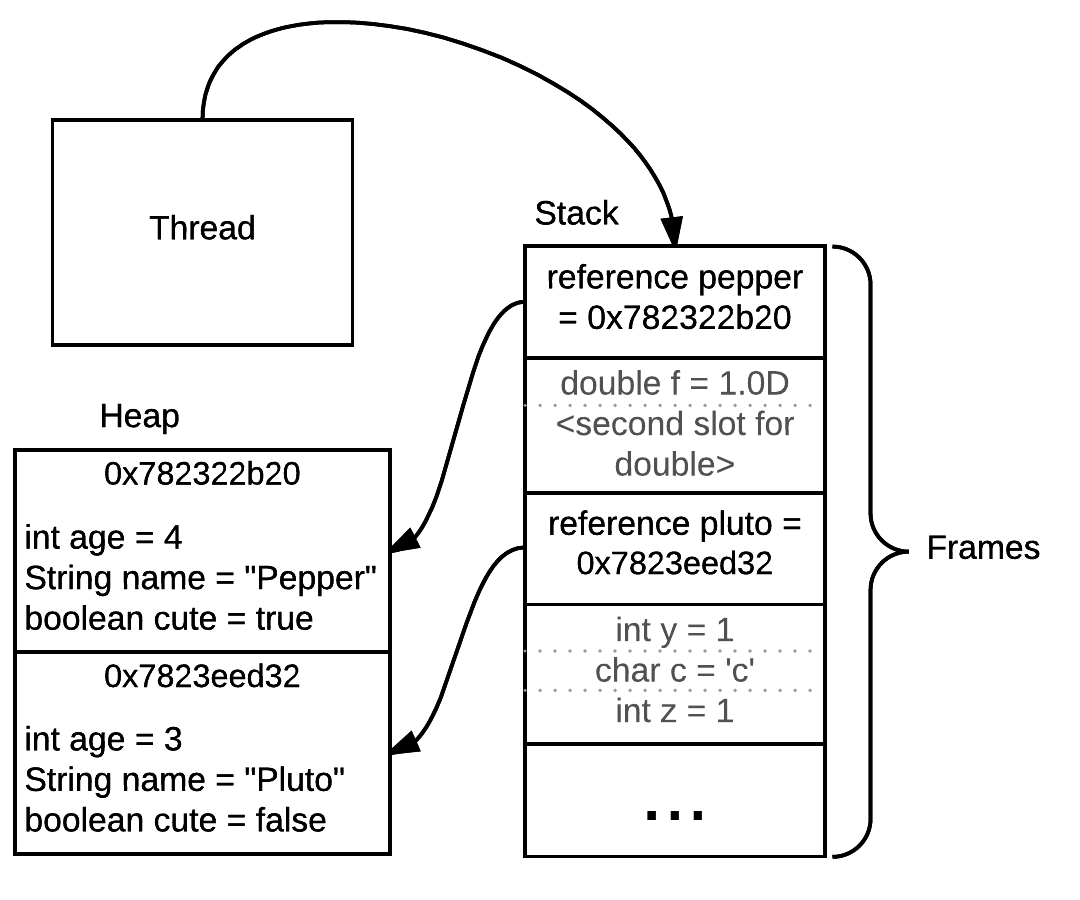
\includegraphics[width=0.9\linewidth]{images/heap}
\caption{The Heap}
\label{fig:stack}
\end{figure}
\subsubsection{String Storage} in Java is represented by sequences of Unicode code points. String is a sequence of characters, which each is represented by two bytes. 

a Java String is a special creature. You can create it as a literal:
\begin{lstlisting}[language=Java]
String literalStr = "test";
\end{lstlisting}
or as an Object:
\begin{lstlisting}[language=Java]
String newStr = new String("test");
\end{lstlisting}

In both cases the reference to it is stored in the stack, the actually string data is in the heap.

Those two strings are additionally curious, though. The literal string is created as an internal string. That means that there is only one copy of the literal string.

Consider the following
\begin{lstlisting}[language=Java]
String newStr      = new String("test");
String newStr2     = new String("test");
String newStr3     = newStr;
String literalStr  = "test";
String internalStr = newStr.intern();
\end{lstlisting}

We can compare these strings in two ways. We can see if the actual characters are the same, or if they actually are the same object (the reference in the stack points to the same spot in the heap).

Comparing newStr and newStr2:
\begin{lstlisting}[language=Java]
newStr      and newStr2     are  not the same
newStr      and newStr2     are  equal
\end{lstlisting}

We created two objects, with exactly the same contents. They are equal (characters match) but not the same (references do not match).

Comparing newStr and newStr3:
\begin{lstlisting}[language=Java]
newStr      and newStr3     are  the same
newStr      and newStr3     are  equal
\end{lstlisting}

We created one object (newStr) and assigned the same reference to the other (newStr3). The values are equal and also the same. There are two values in the stack that point to the same spot in the heap. Changing the contents of one will also affect the other because they are the same.

Comparing newStr and literalStr:
\begin{lstlisting}[language=Java]
newStr      and literalStr  are  not the same
newStr      and literalStr  are  equal
\end{lstlisting}

They are equal (characters match) but they are not the same, as expected. There are two different strings in the heap.

How about the newStr and the internalStr:
\begin{lstlisting}[language=Java]
newStr      and internalStr are  not the same
newStr      and internalStr are  equal
\end{lstlisting}

Just like the previous comparison with the literalStr, internalStr is equal to newStr, but they are not the same.

Now the interesting test, literalStr and internalStr. Notice how internalStr is created from newStr by requesting its internal representation. The results of the comparison:
\begin{lstlisting}[language=Java]
literalStr  and internalStr are  the same
literalStr  and internalStr are  equal
\end{lstlisting}

They are equal and they point to the same location in the heap.

Strings in Java are immutable. Their values cannot be changed. We can assign a new value to a String reference, though. In effect, the string changes, but it really points to a new location in the heap.

The exact location of the internal (literal) strings in the heap used to be different. In Java7 it data changed\cite{java7}:

\begin{quotation}
In JDK 7, interned strings are no longer allocated in the permanent generation of the Java heap, but are instead allocated in the main part of the Java heap (known as the young and old generations), along with the other objects created by the application. This change will result in more data residing in the main Java heap, and less data in the permanent generation, and thus may require heap sizes to be adjusted. Most applications will see only relatively small differences in heap usage due to this change, but larger applications that load many classes or make heavy use of the String.intern() method will see more significant differences.
\end{quotation}


\subsubsection{Storing an Array of ints or Objects}
An Array is an Object that contains other things that are homogeneous. All items in an Array must be of the same type. An Array could, for example, contain ints or Objects (of the same type). 

Regardless of what is stored in the Array, because it is an Object, it is stored like an Object. A reference to it is in the stack, and the actual contents are in the heap.
\subsection{List of Strings}
\textit{Write an application to find out how many total characters can be held in a list of strings before you run out of memory}

The number of characters we can store in a list depends on many factors; the length of the strings, are they String literals or different objects, or the size of the heap. 

\subsubsection{Size of a String}

Java doesn't have a sizeof() functionality like C has, but we can estimate the size of objects in the heap. For a Java String, two bytes are used for each character. There is a bit of overhead (which varies depending on whether the OS is a 32 or 64-bit architecture, for example), and rounding to the next usable memory boundary.

So, a String of 200 characters is approximately 440 bytes in memory (200*2bytes + 38 overhead, and rounded to the closest 8-bit boundary). And empty String (with just overhead) is 40 characters.

We can query the size of the heap, and the amount of free memory:
\begin{lstlisting}[language=Java]
long totMem = Runtime.getRuntime().totalMemory();
long freeMem = Runtime.getRuntime().freeMemory();
\end{lstlisting}

If we request garbage collection (although not guaranteed), allocate Strings of 200 characters until we run out of memory (7,480,318 strings in my example program), the result of the heap is:

\begin{table}[!htb]
\centering
\begin{tabulary}{\columnwidth}{ |>{\raggedright\arraybackslash} p{0.5\columnwidth} | >{\raggedright\arraybackslash}r |}
\hline
Used memory before  & 356,352 bytes \\ \hline 
Used memory after & 3,321,618,024 bytes \\ \hline 
Delta & 3,321,261,672 bytes\\ \hline 
Number of strings  & 7,480,318 \\ \hline
Heap per a string & 444 bytes \\ \hline 
\end{tabulary}
\caption{Java Primitive Types}\label{tab:java-primitive-types}
\end{table}

\subsubsection{Heap and Stack Exceptions}
There are several types of exceptions related to running out of heap or stack.

A java.lang.StackOverflowError is thrown when we run out of stack space. This can occur when we make too many method calls (add too many frames) recursively. In these String List examples, we will not likely run into this problem.

A java.lang.OutOfMemoryError is thrown when we run out of heap, or when the garbage collection cannot efficiently release more heap memory. It is guaranteed to be thrown before we actually run out of heap. The error message can give us more information why the error was thrown. "Java heap space" message means that we truly ran out of heap. "GC overhead limit exceeded" message means that the garbage collection is making poor progress. We get that error if "the Java process is spending more than approximately 98\% of its time doing garbage collection and if it is recovering less than 2\% of the heap and has been doing so far the last 5 (compile time constant) consecutive garbage collections" \cite{gosling}.

If we create a lot of small Strings, we could run into the issue of garbage collection being inefficient before actually running out of heap.

\subsubsection{Heap Size}

The default size of the heap is at most 1GB. If one quarter of the physical memory is smaller than 1GB, then that value is used\cite{gcergo}. A MacBook Pro with 16GB of physical memory:
\begin{lstlisting}[language=Java]
OperatingSystemMXBean mxbean = (OperatingSystemMXBean) ManagementFactory.getOperatingSystemMXBean();
System.out.println(mxbean.getTotalPhysicalMemorySize()/1024/1024);
// 16384
\end{lstlisting}

One fourth of that is 4GB. In this case, because one quarter of the physical memory is larger than 1GB, the default heap is the smaller value, or 1GB.

The maximum heap size on a MacBookPro:
\begin{lstlisting}[language=bash]
$ java -XX:+PrintFlagsFinal -version 2>&1 | grep MaxHeapSize
uintx MaxHeapSize := 4294967296 {product}
\end{lstlisting}
So, approximately 4.29GB. 

\subsubsection{Test Program}
I wanted to test several cases. I wanted to use small Strings (5 characters), medium Strings (100 characters), large Strings (1000 characters), and a random mix of lengths (1-1000 characters). I also wanted to test with internal Strings (literal) and dynamic Strings (created with the new keyword). So, my test cases are:
\begin{itemize}
\item Small  literal Strings
\item Small dynamic Strings
\item Medium literal Strings
\item Medium dynamic Strings
\item Large literal Strings
\item large dynamic Strings
\item Random literal Strings
\item Random dynamic Strings
\end{itemize}

See the source code for the test in Appendix B, page \pageref{App:AppendixB}.

\subsubsection{The Results}
The first test involved using internal (literal) Strings of different sizes. The actual String data is exactly the same copy. In practice, this is a useless example, but it is nevertheless interesting. 

We have a reference to the List in the stack. The List has references to the String items. The List object grows to fill the entire heap until we get an OutOfMemoryError. We don't run out of the stack so we never get a StackOverFlowException.

The results of adding literal strings to a list:
\begin{table}[!htb]
\centering
\begin{tabulary}{\columnwidth}{ | r | r | r |}
\hline
\textbf{Length} & \textbf{Strings}& \textbf{Chars}\\ \hline 
5 & 287,568,537 & 1,437,842,685 \\ \hline
200 & 287,568,537 & 57,513,707,400 \\ \hline
1000 & 287,568,537 & 287,568,537,000 \\ \hline
\end{tabulary}
\caption{List of Literal Strings}\label{tab:listOfLiteralStrings}
\end{table}

We can see that because there is only one exact copy of the actual String data and the List just contains references to the exact same String, the heap runs out of memory with exactly the same number of items in the List, regardless of the String size. The number of items in the List is constant. Because of the size of the String doesn't matter when using a literal String, we can "fit" more characters in the List if the Strings are bigger.

The results of adding dynamic strings to a list:
\begin{table}[!htb]
\centering
\begin{tabulary}{\columnwidth}{ | r | r | r |}
\hline
\textbf{Length} &  \textbf{Strings}& \textbf{Chars} \\ \hline 
5 & 55,591,797 & 277,958,985 \\ \hline
200 & 7,480,318 & 1,496,063,600 \\ \hline
1000 & 1,631,552 & 1,631,552,000 \\ \hline
1-1000 & 3,194,418 & 1,594,871,852 \\ \hline
\end{tabulary}
\caption{List of Dynamic Strings}\label{tab:listOfDynamicStrings}
\end{table}

With dynamic Strings, we can see that as the size of the String gets bigger, the number of items in the List gets smaller. The List full of small Strings holds the least number because most of the heap is used for String overhead. The List with random length Strings is logically between a list of 200-character-String List and 1000-character-String List.

\subsubsection{Overhead Ratio}
There is a point where the overhead becomes less and less relevant. As the String size grows, the number of characters, or Strings, becomes practically linear. 
\pgfplotsset{width=0.75\columnwidth,compat=1.3}\\

\begin{figure}[H]\centering
\begin{framed}
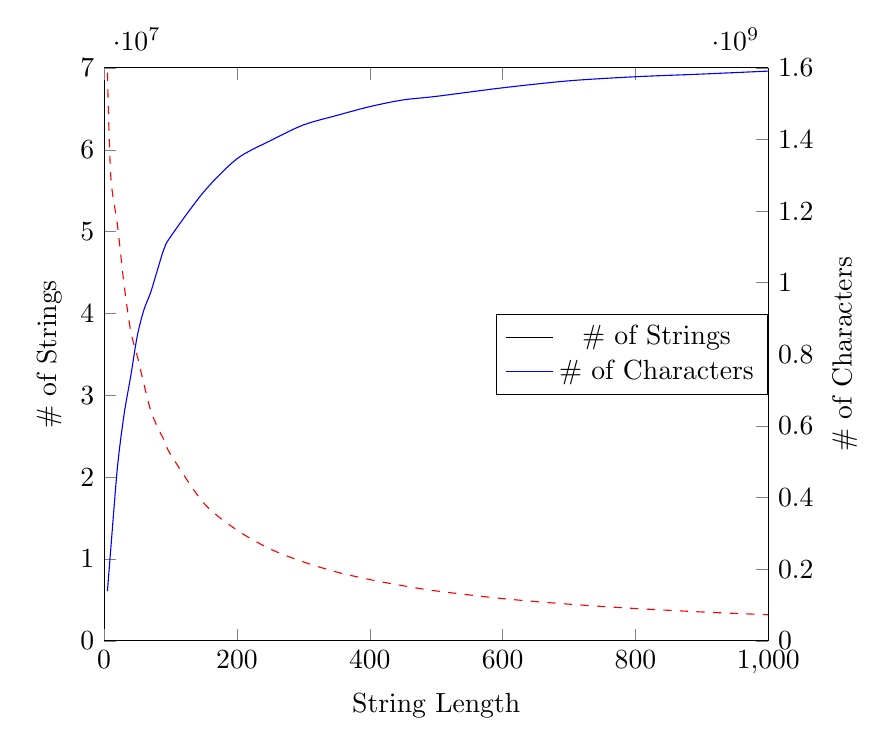
\begin{tikzpicture}
\pgfplotsset{
    scale only axis,
%    	xmajorgrids,
    xmin=0, xmax=1000,
    legend style={at={(1,0.5)},anchor=east}
}
\begin{axis}[
    axis y line*=left,
    axis x line=none,
    ylabel={\# of Strings},
    ymin=0, ymax=70000000
]
% # of strings
\addplot[color=red, only marks, smooth,dashed]
    coordinates {
(5,   69429204)
(10,  56803662)
(20,  50864895)
(30,  43559683)
(40,  37869108)
(50,  34779731)
(60,  31345545)
(70,  28185086)
(80,  26173543)
(90,  24571971)
(100, 22794732)
(150, 16830715)
(200, 13527266)
(250, 11220477)
(300,  9636571)
(350,  8407166)
(400,  7480318)
(450,  6729742)
(500,  6095017)
(600,  5154652)
(700,  4474650)
(800,  3945494)
(900,  3521442)
(1000, 3184637)

    };
    \label{strings_plot}
\addlegendentry{\# of Strings}

\end{axis}

\begin{axis}[
    axis y line*=right, 
    xlabel={String Length},
    ylabel={\# of Characters},
%    	ymajorgrids,
    ymin=0, ymax=1600000000
	]
\addlegendimage{/pgfplots/refstyle=strings_plot}\addlegendentry{\# of Strings}
% # of characters
\addplot[color=blue, only marks, smooth]
    coordinates {
(5,   138860440)
(10,  255609450)
(20,  483226293)
(30,  631621316)
(40,  738473565)
(50,  852200636)
(60,  924632662)
(70,  972560340)
(80,  1033822001)
(90,  1093504365)
(100, 1128493640)
(150, 1253741942)
(200, 1346137653)
(250, 1396506412)
(300, 1440740739)
(350, 1467137115)
(400, 1491908107)
(450, 1510647853)
(500, 1520613428)
(600, 1544464935)
(700, 1564055520)
(800, 1575428971)
(900, 1582875340)
(1000,1591165537)
    };
 \label{characters_plot}
\addlegendentry{\# of Characters}
\end{axis}
\end{tikzpicture}
\end{framed}
\caption{Number of Characters in a List by String Length}
\label{fig:listofstrings}
\end{figure}
\pgfplotsset{width=\columnwidth,compat=1.3}

My program threw a heap exception when the heap was at 3.09GB. The exception is guaranteed to be thrown before the heap actually runs out, though.

With that heap size, the number of characters approaches 1,600,000,000, which seems close to the maximum number of characters I can store in a List of Strings (with this heap size).

The number of Strings in the List approaches 3,000,000.

When the String length is greater than about 200, the overhead seems to get less and less in the way.
\subsection{StringBuffer vs StringBuilder}
\textit{Compare and contrast StringBuffer and StringBuilder and when to use each}
StringBuffer and StringBuilder have identical APIs. The main difference between them is that a StringBuffer is thread-safe and StringBuilder is not.

StringBuffer is the older of the two and was created with synchronization so it could be used by several threads. In practice, it is hard to find a real use case for that. In theory, StringBuilder, that is not thread-safe, is faster because it doesn't have to worry about concurrency.

\subsubsection{Concurrent Writes}
I wrote a simple program that Creates two threads that write into a StringBuilder and a StringBuffer 10 times. See appendix C on page \pageref{App:AppendixC}.

The thread writes into the buffer, then into the builder, and then sleeps for 10ms. In the end it prints out the contents of the StringBuilder and the StringBuffer:
\begin{lstlisting}
Buffer	Builder
0:0     1:0
1:0     0:0
0:1     0:1
1:1     1:1
0:2     ????0:2
1:2     1:3
1:3     0:3
0:3     1:4
1:4     0:4
0:4     1:5
1:5     0:5
0:5     1:6
1:6     0:6
0:6     1:7
1:7     0:7
0:7     1:8
1:8     0:8
0:8     1:9
1:9     0:9
0:9     
\end{lstlisting}

The contents of the StringBuilder and StringBuffer are different. Not only is the order different but the StringBuilder seems to be missing a line. Thread 1, iteration 2 is missing in the StringBuilder output. Instead there are non-printing characters (shown as '?').

Looking at the bytes in the StringBuilder shows the issue.

Each line consists of four characters; the thread name (really a number from 0 to 9), a colon, and the counter value (from 0 to 9), and a new line character, like this:
\begin{lstlisting}
31 3a 30 0a    1:0.
\end{lstlisting}
The StringBuilder contains exactly four bytes of 0's, though, starting in position 10 (second line in the following listing)
\begin{lstlisting}
0000000: 313a 300a 303a 300a 303a 310a 313a 310a
0000010: 0000 0000 303a 320a 313a 330a 303a 330a
0000020: 313a 340a 303a 340a 313a 350a 303a 350a
0000030: 313a 360a 303a 360a 313a 370a 303a 370a
0000040: 313a 380a 303a 380a 313a 390a 303a 390a
\end{lstlisting}

It looks like the two threads collided. Thread 1 reserved 4 bytes in the StringBuilder, but thread 2 wrote its output. This clearly shows how StringBuilder is not thread safe.

\subsubsection{Comparison Test}
I compared appends to a StringBuffer and a StringBuilder to see which one is faster. I used different lengths of strings and different number of additions. See appendix D on page \pageref{App:AppendixD}.

I appended strings of 1, 5, 10, 25, and 50 characters long into a StringBuffer or a StringBuilder. I appended from 1,000,000 to 10,000,000 strings per run, in increments of 1,000,000 strings.

In the graph below, we can see that as for both the StringBuffer and the StringBuilder, when the size of the string to append increased, the time increased also. Even greater was the time increase as the number of additions grew. In those aspects both the StringBuffer and the StringBuilder behaved similarly.

Suprisingly, appending into a StringBuilder was not always faster than into a StringBuffer. In the graph, the blue plane is the data of appending into a StringBuffer. The red dots show when appending into a StringBuilder was slower. Although the difference is not great, there is no clear pattern of why the StringBuilder was slower sometimes.

\pgfplotstableread{buffer.txt}{\plotdata}
\begin{figure}[H]\centering
\begin{tikzpicture}
  \begin{axis}[view/h=40, grid=both, xlabel={String Size}, ylabel={Additions ($10^7$)}, zlabel={Time (ms)}, ylabel shift=-15pt, xlabel shift=-10pt, zlabel shift=-6pt,ytick scale label code/.code={}]
\addplot3[surf, opacity=0.8, colormap=
    {blackblue}{color=(blue) color=(blue)}] file {buffer.txt};    
    \addplot3[red!80,mark=*,
mark options={fill=red!80!red},
only marks,mark size=1pt] file {builder2.txt};    
  \end{axis}
\end{tikzpicture}
\label{fig:stringbuildervsStringBuffer}
\end{figure}

\subsection{Collections}
\textit{Compare/contrast use of ArrayList / LinkedList / HashMap / HashSet / TreeSet}
Notes: write sample application to show the use of the collections. Check for execution times
Make a table for comparison

some text

\subsection{Sorting in Order}
\textit{Write an application to read a file with 10k lines of text, and output another file with the lines in sorted order.}

some text

\subsection{Sorting in Reverse Order}
\textit{Write an application to read a file with 10k lines of text, and output another file with the lines in reverse sorted order}

After sorting the file in order, reversing the order is trivial.

For the in-memory solution, we can just reverse the comparator:

\begin{lstlisting}
33c33
<  return left.compareTo(right);
---
>  return right.compareTo(left);

\end{lstlisting}
So, we compare the right element to the left. The rest of the code is the same as in order sorting. See Appendix G on page \pageref{App:AppendixG} for the class \texttt{ReverseSortInMemoryExample.java}.

\subsubsection{Sorting, in Reverse Order, a File That is Too Big}
Similarly, sorting a large file in reverse order requires just a minor change.

\begin{lstlisting}
105c105
<  if (lowest.getValue().compareTo(entry.getValue()) > 0) {
---
>  if (lowest.getValue().compareTo(entry.getValue()) < 0) {
165c165
<  return left.compareTo(right);
---
>  return right.compareTo(left);

\end{lstlisting}

The sorting of the partial files changed, just like in the in-memory version. In addition the merge change to pick the last String in order, instead of the first.

See Appendix G on page \pageref{App:AppendixG} for the class \texttt{SortReverseInFileExample.java}.
\subsection{Exceptions}
\textit{Write code to show exception handling including examples of checked, unchecked, and Error exceptions}

Errors and exceptions are unexpected conditions that may occur in the course of running a program. There is a mechanism in the Java language that allows us to alert of an error and handle it outside the normal logical flow of the program.

\begin{description}
\item[Throwable] The top-level class for handling errors and exceptions. It inherits from Object. It captures the stack trace.
\item[Stack trace] A list of locations (line numbers) and descriptions of where the error or exception occurred.
\item[Error] A "serious problem that a reasonable application should not try to catch"\cite{error}. These are errors that a programmer has no control over, and if encountered, there is nothing that the programmer can do to overcome it.
\item[Exception] "Indicates conditions that a reasonable application might want to catch" \cite{exception}. A programmer should try to anticipate these kinds of issues and handle them without the program terminating.
\item[try] A block that contains code that might throw an exception.
\item[throw] To raise an exception. When a piece of code needs to alert about an issue it it said to "throw an exception".
\item[catch] When a piece code handles an issue, it is said to "catch the exception".
\item[finally] A block of code that is executed after an exception is thrown or handled, regardless if it is handled or not.  Finally block is optional. It is useful for cleaning up resources, for example, because it is executed always, regardless of an error or not. If we, for example, close a file in the try block and there is an exception before it gets to that line, the file will not be explicitly closed. On the other hand, if we close the file in the finally block, it will be executed even if there is an exception.
\end{description}


\begin{figure}[!h]\centering
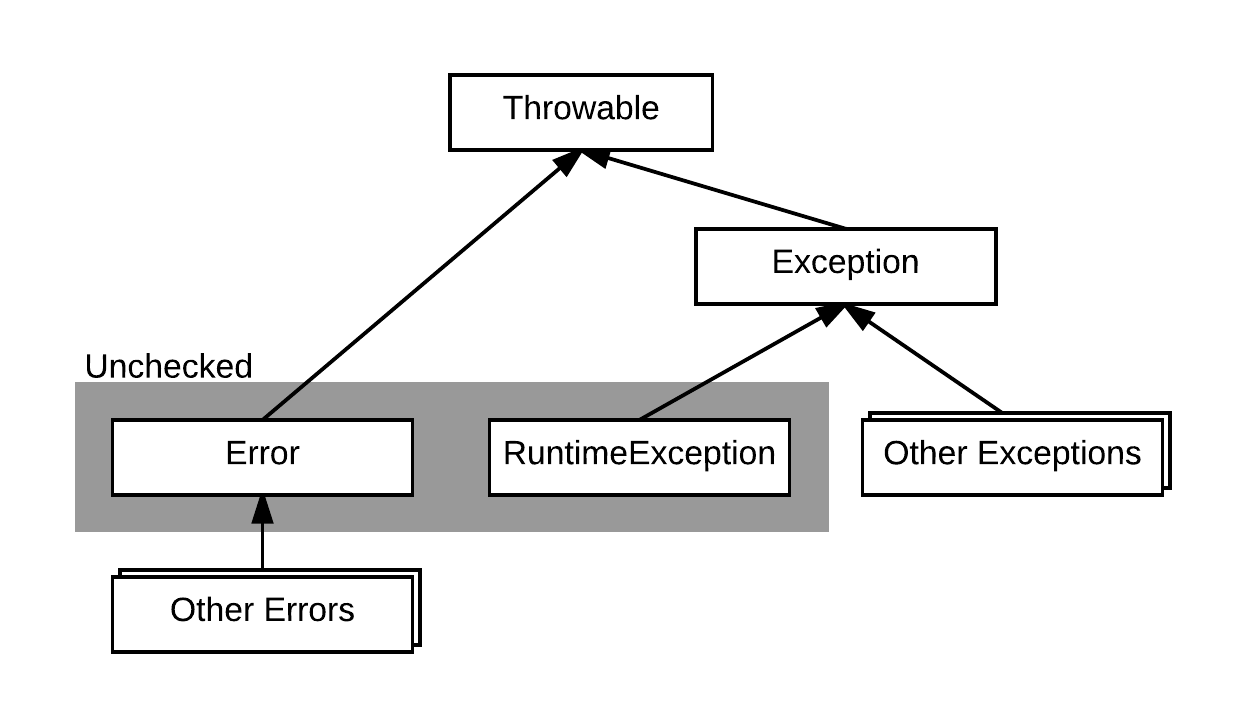
\includegraphics[width=\linewidth, frame]{images/exceptionhierarchy}
\caption{Exception Hierarchy}
\label{fig:exceptions}
\end{figure}

There are two types of \texttt{Exceptions}; checked and unchecked.

\subsubsection{Checked or Uncecked}
Any exception that is a subclass of \texttt{RuntimeException}, a special subclass of \texttt{Exception}, is a so-called "unchecked" exception. All \texttt{Error} subclasses are also unchecked exceptions. There is nothing that the user would reasonable be able to do to overcome them. These exceptions will not generate a compiler error, so that they will not end up cluttering the code unnecessarily. The programmer can completely ignore them, not even plan to catch them at all. \cite{runtimeexception} If we don't catch them, they will bubble up and interrupt the control flow. Eventually the JVM will display the error in the console, and quit.

The checked exceptions are the ones that generate a compiler error if not handled.

When a user of the code is reasonable expected to recover from a exception, we should use checked exceptions. If not, use unchecked exceptions.\cite{runtimeexception}

\subsubsection{Pitfalls}

Using exceptions to control flow is the most common pitfall with error handling. We should not rely on an exception to occur to make decisions on what to do next. Exceptions are just that, exceptions.

In an encapsulated design, though, there are some difficulties. Imagine a method that returns a Dog object, for example. What if the user didn't provide a name for the dog when we instantiate it? Should the code allow creation of a dog without a name? If so, how do we tell the user that the name is required? We can only return a Dog object, so we couldn't replace it with an error object. We could return a Dog object and have it include an error field. The user would be required to check if there is a value in the error field. Or we could put the error in the name field. Another way could be that we have a global error field and if there is an error we store the message there.These are all bad ideas and go against encapsulation and good object-oriented principles. The solution is to throw an exception. The user doesn't get a Dog object back. Instead there is an exception. The user of the method then has to either handle it or ignore it.

These considerations are made at the time of writing the program although, the exceptions occur at the runtime.

\subsubsection{A Specialized Exception}
Usually the Java provided exception classes are sufficient for handling most of the conditions that might arise in a program. There is little need for creating specialized exceptions. Some programmers just like to have all exceptions be their own in a program. When there is an invalid parameter, for example "\@\$\#\%\$*\&" passed into a dogs name, they want to  throw a "\texttt{MyApplicationException}". A better choice would be an existing  \texttt{IllegalArgumentException} instead.

There are some cases, though, when it might be convenient. Imagine a method that wants to return an error code in case of an exception. That code can be used to easily localize the error message shown to the user. 

In order to create our own exception class, we would extend either \texttt{Exception} or \texttt{RuntimeException} (checked or unchecked).
\begin{lstlisting}[language=Java]
public class MyException extends Exception {
// ...
}
\end{lstlisting}

We then would add a field for the error code. 
\begin{lstlisting}[language=Java]
private int errorCode;

public int getErrorCode() {
 return errorCode;
}

public void setErrorCode(int errorCode) {
 this.errorCode = errorCode;
}

@Override
public String getMessage() {
 return super.getMessage() + " (" + errorCode + ")";
}
\end{lstlisting}

We would then override all constructors and let the user pass in the error code. In those constructors we would call the corresponding super constructor and  initialize the error code field. 
\begin{lstlisting}[language=Java]
public MyException(int errorCode) {
 this.errorCode = errorCode;
}

public MyException(Throwable cause, int errorCode) {
 super(cause);
 this.errorCode = errorCode;
}

public MyException(String message, int errorCode) {
 super(message);
 this.errorCode = errorCode;
}

public MyException(String message, Throwable cause, int errorCode) {
 super(message, cause);
 this.errorCode = errorCode;
}
\end{lstlisting}


See Appendix H (MyException.java) on page \pageref{App:AppendixHExeption} for the full source of a sample custom exception.


\subsubsection{Throwing an Exception}
When we have a need to alert about an issue we throw an exception. In order to do that we need to consider two things
\begin{lstlisting}[language=Java, label=lst:throwException]
private void throwCustomException() 
   throws MyException {
 if (someConditionIsTrue) {
   throw new MyException("My message", 404);
  } else {
   System.out.println("Don't throw it...");
  }
}
\end{lstlisting}

We need to add a \texttt{throw} statement where we need to alert about the error, line 4 in listing \ref{lst:throwException}. Also, for checked exceptions, we need to add a \texttt{throws} statement in the method signature (line 2). For unchecked exceptions we don't need to add anything to the method signature.

\subsubsection{Handling an Exception}
When we call a method that throws an exception, we may want to choose to handle it. 

\begin{lstlisting}[language=Java, label=lst:catch]
try {
  throwCustomException();
} catch (MyException e) {
  System.out.println(e.getMessage());
} finally {
  System.out.println("Finally");
}
\end{lstlisting}

We enclose the method that throws an exception in a \texttt{try} block, lines 1-3 of listing \ref{lst:catch}. We have a \texttt{catch} block that handles the exception (lines 3-5). We also have an optional \texttt{finally} block that is executed after the catch block (lines 5-7).

On the other hand, if we choose not to catch an exception, we can propagate it by adding a \texttt{throws} statement in the method signature (line 6 in listing \ref{lst:propagate}).

\begin{lstlisting}[language=Java, label=lst:propagate]
/**
  * We don't catch it, just let it propagate up.
  * If it is a checked exception, someone higher
  * up will eventually have to catch it
  */
private void catchCustomException() throws MyException {
  throwCustomException();
}
\end{lstlisting}

See full listing of the code in Appendix H (ExceptionExample.java)on page \pageref{App:AppendixHExample}.
\subsection{Enums}
\textit{Write your own enum type.  Describe when you would use it.}

An \texttt{enum} is a special object that looks like a constant. They are useful when we need a list of constants that are not numeric. For example, types of things are well represented as an \texttt{enum}, such as representing a gender of a person. Instead of having numbers (0=unknown, 1=male, 2=female) or \texttt{String}s ("unknown", "male", or "female") we should use an \texttt{enum}. If we use numbers or \texttt{String}s, for example, we don't have control over the possible values that the user might assign to the value. What would we do it someone assigns 99 to gender (\texttt{int})? If we chose to do that, we would need extra logic to verify the value. Also, the user doesn't know which values are valid before trying it, or reading the documentation.

\subsubsection{A Simple Enum}
A simple \texttt{enum} is basically a list of names:
\begin{lstlisting}[language=Java]
public enum NaughtyOrNice {
  REALLY_NICE,
  NICE,
  NOT_SO_NICE,
  AVERAGE_NICE,
  NOT_REALLY_NAUGHTY,
  NAUGHTY,
  REALLY_NAUGHTY
}
\end{lstlisting}

Each \texttt{enum} value is assigned an ordinal (\texttt{int}). This value can be retrieved, but it cannot be set. We shouldn't rely on the ordinal value, as it might change when we add or remove \texttt{enum} values.

\begin{lstlisting}[language=Java]
NaughtyOrNice status = NaughtyOrNice.AVERAGE_NICE;
System.out.println(status + ":{\n"
 + " name:'" + status.name() + "',\n"
 + " ordinal:'" + status.ordinal() + "'\n" +
 "}");

if (peterStatus.equals(NaughtyOrNice.REALLY_NAUGHTY)) {
 System.out.println("He has no hope");
} else {
 System.out.println("He has some hope");
}
\end{lstlisting}

When run, the above code will produce:
\begin{lstlisting}
AVERAGE_NICE:{
 name:'AVERAGE_NICE',
 ordinal:'3'
}
He has some hope
\end{lstlisting}

\subsubsection{A Custom Enum}
There are cases when we want the \texttt{enum} to have values associated to it. For example, we might want to associate strings with an \texttt{enum} for parsing or displaying.

A custom \texttt{enum} looks like a class, except that it its type is \texttt{enum} not \texttt{class}.

\begin{lstlisting}[language=Java]
public enum ErrorType {
 //...
 
 public int getErrorCode() {
  return errorCode;
 }

 public String getErrorMessage() {
  return errorMessage;
 }

 @Override
 public String toString() {
  return this.name() + ": {\n"
   + " ordinal:'" + ordinal() + "',\n"
   + " msg:'" + errorMessage + "',\n"
   + " code:'" + errorCode + "'\n" +
   "}";
 }
}
\end{lstlisting}

Declaring the possible values is done in a strange way too, inside the \texttt{enum} itself:
\begin{lstlisting}[language=Java]
E404(404, "Not Found"),
E500(500, "Really Bad Error"),
UNKNOWN(0, "Unknown");
\end{lstlisting}
In the above example, we declare the name of the \texttt{enum} value (E404, for example), then pass in any parameters to the constructor. In this case we assign a numeric error code (404) and a message string "Not Found".

See the source for the custom \texttt{enum} in Appendix I (ErrorType.java) on page \pageref{App:AppendixIEnum}.

Sometimes it is useful to map a literal value with an \texttt{enum}. For example, if we get an error from an API in form of a number, we might want to map it into an \texttt{enum}. Unfortunately this is not provided. The following code shows how to do it:
\begin{lstlisting}[language=Java]
public static ErrorType fromValue(int errorCode) {
 ErrorType[] values = ErrorType.values();
 for (ErrorType value : values) {
  if (value.getErrorCode() == errorCode) {
   return value;
  }
 }
 return UNKNOWN;
}
\end{lstlisting}
The code iterates through the values of the \texttt{enum} and picks the one that matches the given input. If none is found, then it defaults to \texttt{UNKNOWN}.

To convert a numeric value into an \texttt{enum} can then be done:
\begin{lstlisting}[language=Java]
ErrorType error500 = ErrorType.fromValue(500);
System.out.println(error500);
\end{lstlisting}

The output will be:
\begin{lstlisting}
E500: {
 ordinal:'1',
 msg:'Really Bad Error',
 code:'500'
}
\end{lstlisting}

\subsubsection{Switching on an Enum}
We can use \texttt{enums} in a switch statement:
\begin{lstlisting}[language=Java]
String msg;
switch (myError) {
 case E404:
  msg = "Where did it go?";
  break;
 case E500:
  msg = "Let's just give up";
  break;
 default:
  msg = "Who knows?";
  break;
}
\end{lstlisting}
However, the syntax is a bit restricted. For example You cannot use a fully qualified \texttt{enum}
\begin{lstlisting}[language=Java]
case ApplicationError.E404:
\end{lstlisting}
Although this is valid in an if statement, for example, this causes the compiler to complain that the case label is not a constant. The proper way is:
\begin{lstlisting}[language=Java]
case E404:
\end{lstlisting}
Also wrapping the cases in parentheses is not valid.
\begin{lstlisting}[language=Java]
case (E404):
\end{lstlisting}
The above listing generates an error "Constant expression required". Parentheses around an \texttt{int} case label, for example is valid syntax. Not when it comes to enums.

See full listing in Appendix I (EnumExample.java) on page \pageref{App:AppendixIExample}
\section{Methods, Encapsulation and Inheritance}

some description
\subsection{Composition, Inheritance, and Static Methods}
\textit{Show how to use a common piece of logic from two different classes, in three different ways: 1) by composition, 2) by inheritance, and 3) by static method calls, discuss the tradeoffs.}

\subsubsection{Inheritance}\label{s:inheritance}
The easiest way to think of class inheritance is that it is an "is-a" relationship. One class (child class) "is a" type of another class (super class).

For example, Cat and Dog classes are not the same, but they share common features. Both cats and dogs make a sound and they probably have a name. They have legs. We can abstract that common functionality into a super class called Animal.

\begin{figure}[H]\centering % Using \begin{figure*} makes the figure take up the entire width of the page
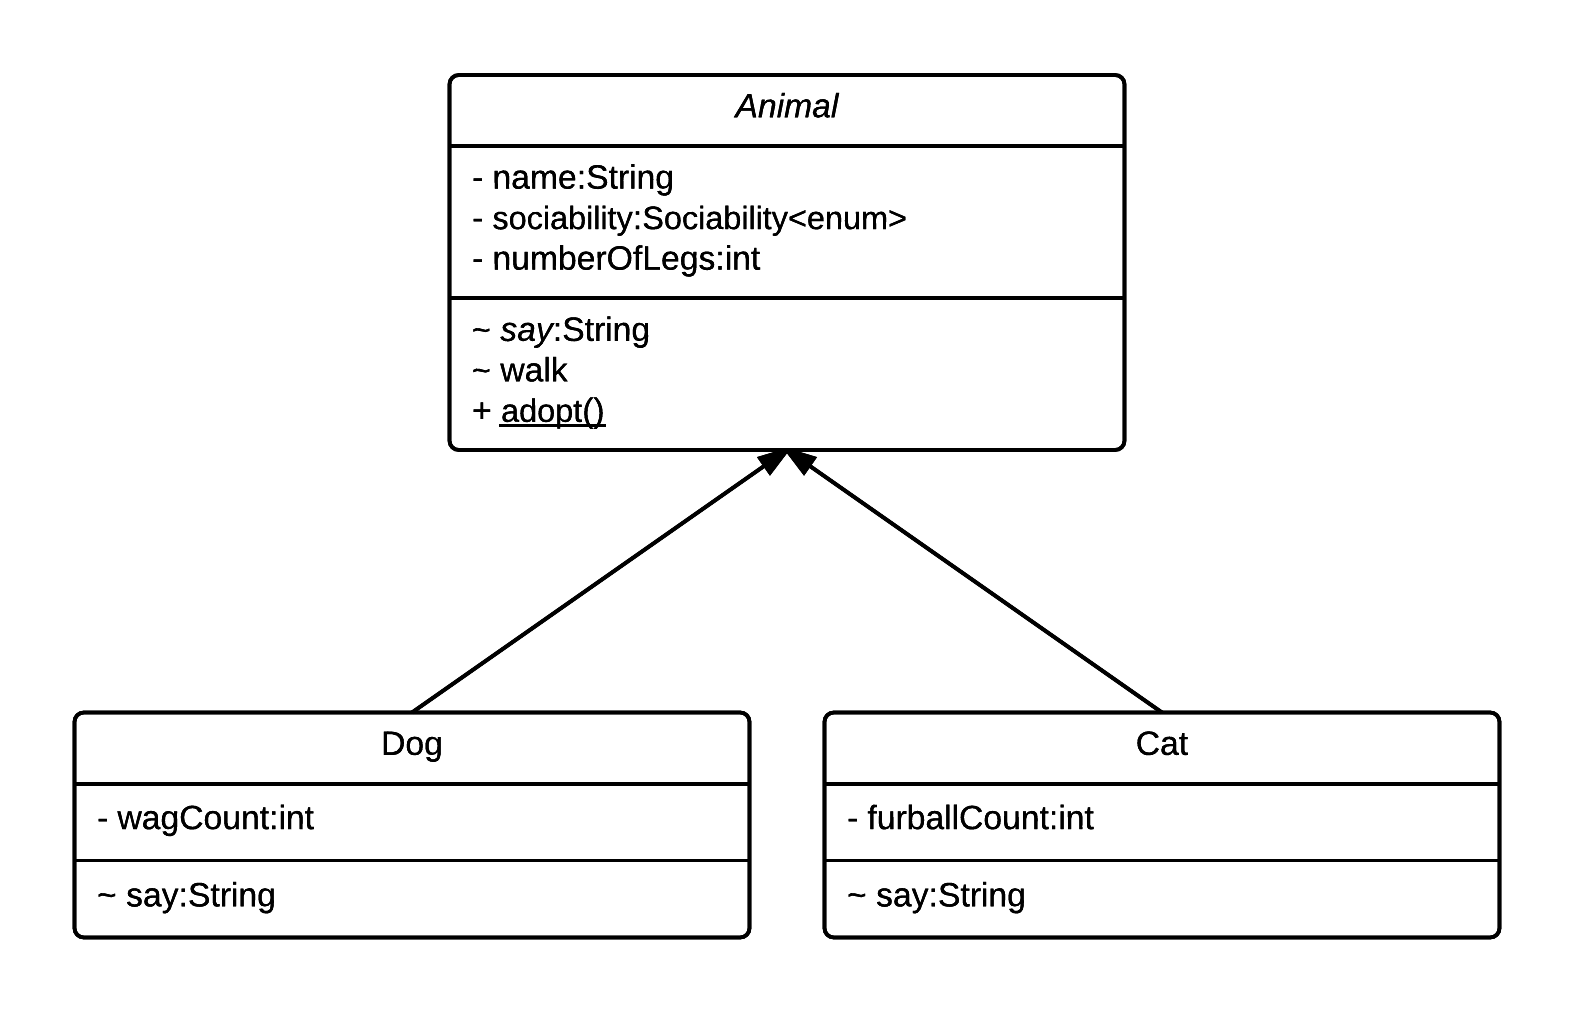
\includegraphics[width=0.9\linewidth, frame]{images/inheritance}
\caption{Inheritance ("Is-a")}
\label{fig:inheritance}
\end{figure}

A Dog "is-a" Animal. The Cat "is-a" Animal. They inherit all package public, protected, and public methods and fields of Animal.

If the super class has any public or package public methods, the child classes can call them. For example, if Animal has a method walk:
\begin{lstlisting}[language=Java]

void walk() {
    String steps = this.getName() + " walks: ";
    for (int i = 0; i < numberOfLegs; i++) {
      steps += " step";
    }
    System.out.println(steps);
  }

\end{lstlisting}

We can call it from the Dog and Cat classes, as we did in the say method. There is no way to force Dog call the walk() method. If there is something that we want to enforce, there is a better way.

In Animal we have specified an abstract method say(). This way we force an Animal to have that functionality, but we let the child classes to specify what it means. 

\begin{lstlisting}[language=Java]
 public abstract String say();
\end{lstlisting}

Although they both say things, they say different things. Dogs bark and cats meow.
In order to do this, we also mark the Animal class abstract. That means that the user cannot create an instance of an Animal. We can only create instances of the child classes that are not abstract and implement the say method. This way we force the child classes to implement the say method.

Dog:
\begin{lstlisting}[language=Java]
// Dog:
@Override
  public String say() {
    String whatDoesTheCatSay = "Bark";
    for (int i = 0; i < wagCount; i++) {
      whatDoesTheCatSay += " (wag)";
    }
	super.walk();
    return whatDoesTheCatSay;
  }
  
// Cat:
@Override
  public String say() {
    String whatDoesTheCatSay = "Meouw";
    for (int i = 0; i < furballCount; i++) {
      whatDoesTheCatSay += " (cough)";
    }
    super.walk();
    return whatDoesTheCatSay;
  }
\end{lstlisting}

Providing an alternate implementation of a method in the child class is called overriding. The overriding method has to have the same signature (return type and parameter list) as the method in the parent class. Java provides an annotation for marking a method overridden, namely @Override. If we use it and our method doesn't match the parent method, we will see an error. The annotation is useful for keeping us in check when overriding methods.

Cats and dogs also have unique features.  Cats have fur balls and dogs wag their tails. In the say method, we also add unique features. Dogs wag their tails and cats cough up furballs.

We can now create cats and dogs:
\begin{lstlisting}[language=Java]

Animal pluto = new Dog("Pluto", Animal.Sociability.VERY_SOCIAL, 3);
Animal sheba = new Cat("Sheba", 2);

// We can also create a Dog object
Dog pepper = new Dog("Pepper", Animal.Sociability.VERY_SOCIAL, 99);

\end{lstlisting}

The difference between pluto and pepper is that the pluto reference is of type Animal, and the pepper reference is of type Dog. There usually isn't a good reason to use the specific reference (pepper). It conceptually goes against the purpose of inheritance.

When we call the say method we have the following output:
\begin{lstlisting}[language=Java]
Bark (wag) (wag) (wag)

Person{pets=[{name:' Spot'}, {name:' Sheba'}]}
Sheba walks:  step step step step
Meouw (cough) (cough)
\end{lstlisting}

One of the benefits of inheritance is that we can treat Cat and Dog objects the same way, as instances of the Animal class. With that, we can, for example, store Cats and Dogs in the same collection:
\begin{lstlisting}[language=Java]
Animal sheba = new Cat("Sheba", 2);
Animal spot = new Dog("Spot", Animal.Sociability.VERY_SOCIAL, 5);
List<Animal> pets = new ArrayList<Animal>();
pets.add(spot);
pets.add(sheba);
\end{lstlisting}

See page \pageref{App:AppendixJInheritance} for full source code.

\subsubsection{Composition}

A composition is another way to share features between classes. The easiest way to think of it is a "has-a" relationship. For example, a Cat and a Dog "have-a" Tail.

\begin{lstlisting}[language=Java]
public class Tail {
  private boolean 	;
  private int length;

  public Tail(boolean docked, int length) {
    this.docked = docked;
    this.length = length;
  }
}
\end{lstlisting}

We can make the Animal class "have"a" tail. Because Dog "is-an" animal, it also "has-a" Tail. The same for the Cat.
\begin{figure}[H]\centering % Using \begin{figure*} makes the figure take up the entire width of the page
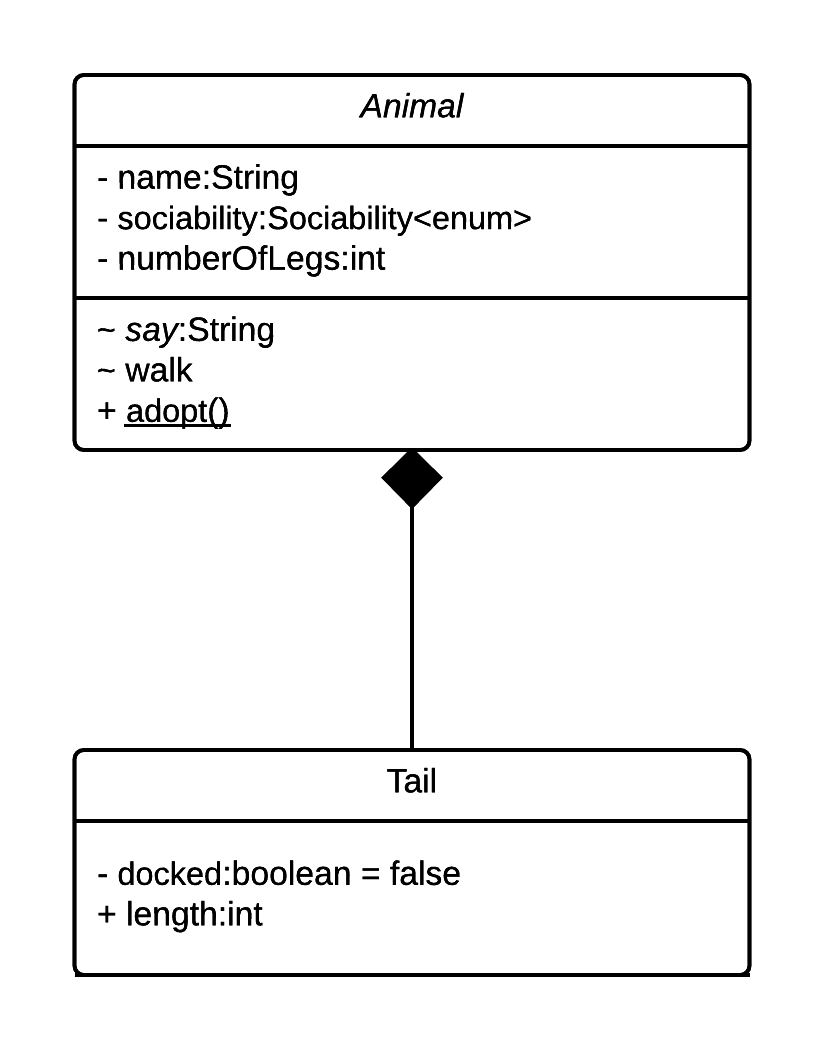
\includegraphics[width=0.9\linewidth, frame]{images/composition}
\caption{Composition ("Has-A")}
\label{fig:composition}
\end{figure}

We just create a field in the Animal class for the tail.
\begin{lstlisting}[language=Java]
private Tail tail;
\end{lstlisting}

Now we can access it from Dog or Cat, as well as from Animal:
\begin{lstlisting}[language=Java]
super.setTail(tail);
\end{lstlisting}

See page \pageref{App:AppendixJComposition} for full source code.

\subsubsection{Static Methods}
There is yet another way to provide common functionality among several classes. We can declare a method or field static:

\begin{lstlisting}[language=Java]
public static String adopt(){
 return "Yay! Adopted Animal!";
}
\end{lstlisting}

The static keyword makes the class, field, or method special. We don't need to instantiate an object to access static members of a class. They are class-level parameters and fields:
\begin{lstlisting}[language=Java]
System.out.println(Animal.adopt());

// displays
Yay! Adopted Animal!
\end{lstlisting}
We can access the static adopt() method from the class, without using the new keyword to create an object.

A class might want to provide static fields, for example constants. In such case they should be also marked final, to avoid modification.

Also anything that we might want to share between objects of the same class should be marked static. For example, we might (for some strange reason) want to keep a count of instances of a class. If we declare a static field, all instances of the class will access exactly the same copy of that field. If one modifies it, it will be also show modified for the other instances.

See page \pageref{App:AppendixJTest} for full source code.

\subsubsection{Inner Classes}
It is worth mentioning one more way of sharing code between classes. In Java we can have inner classes, or classes inside of other classes. They have access to all the fields and methods of the outer class, including the private members.

An inner class can be instantiated from outside the outer class, if its access modifiers are set properly. But, the instantiation has to happen through an object of the outer class:
\begin{lstlisting}[language=Java]
OuterClass outer = new OuterClass();
OuterClass.InnerClass inner = outer.new InnerClass();
\end{lstlisting}

The inner object now has access to everything in the outer class. We could create two or more inner classes this way, and they all have access to common methods and fields in the outer class. 

It is not an "is-a", nor a "has-a" relationship. In some ways it breaks encapsulation and doesn't really look like object-oriented programming at all.
\subsection{Constructors}
\textit{Create and overload constructors -- Create a class that has 4 fields and construct the class with variations of one required field and the others are optional.  Use constructor chaining as an example.}

A Constructor is a special method that is called to create (instantiate) and object from a class. It consists of an access modifier and the name of the Class, followed by parentheses that can have zero or more parameters.

There can be several versions of the Constructor, with different parameter lists. This is called constructor overloading.

A constructor can call the parent class constructor using the keyword super. In fact, the child classes should call the super constructor instead of trying to call setters in the super class. The call to the super constructor must be the first line in the child constructor.

A constructor can also call another version of the constructor in the same class. This is called constructor chaining.

\begin{lstlisting}[language=Java]
public Dog(String name, Sociability sociability, int wagCount, Tail tail) {
  super(name, 4, sociability, tail);
  this.setWagCount(wagCount);
}

public Dog(String name, Sociability sociability, int wagCount) {
  this(name,sociability, wagCount, new Tail());
}

public Dog(String name, Sociability sociability) {
  this(name,sociability, 0);
}

public Dog(String name) {
 this(name,Sociability.SOCIAL);
}
\end{lstlisting}\label{code:constructors} 

Appendix J on page \pageref{App:AppendixJ} contains the source code for the \texttt{Dog.java} class.

There are four constructors in the Dog class. The first one, on line 1,  allows us to set all fields in one call; name, sociability, wagCount, and tail. The other constructors (lines 6, 10, and 14) provide defaults for sociability, wagCount, and tail. All constructors require that we provide the name.

Instead of all constructors calling the super constructor, or setters, we call another constructor in the same class.

We can now create Dogs in different ways
\begin{lstlisting}[language=Java]
Dog sparky = new Dog("Sparky");
Dog harley = new Dog("Harley", Animal.Sociability.SOMEWHAT_UNSOCIAL);
Dog spud = new Dog("Spud", Animal.Sociability.VERY_SOCIAL, 3);
Dog kingkong = new Dog("King Kong", Animal.Sociability.VERY_SOCIAL, 1, new Tail(true, 1));
\end{lstlisting}
Appendix J on page \pageref{App:AppendixJ} contains the source code for the \texttt{InheritanceCompositionExample.java} class.
The output:
\begin{lstlisting}
Animal{
  name='Sparky', 
  sociability=SOCIAL, 
  numberOfLegs=4, 
  tail=Tail{docked=false, length=0}
}
Animal{
  name='Harley', 
  sociability=SOMEWHAT_UNSOCIAL, 
  numberOfLegs=4, 
  tail=Tail{docked=false, length=0}
}
Animal{
  name='Spud', 
  sociability=VERY_SOCIAL, 
  numberOfLegs=4, 
  tail=Tail{docked=false, length=0}
} (wag) (wag) (wag)
Animal{
  name='King Kong', 
  sociability=VERY_SOCIAL, 
  numberOfLegs=4, 
  tail=Tail{docked=true, length=1}
} (wag)
\end{lstlisting}

\subsubsection{The Destructor}
In many languages there is also a destructor, a special method to release the memory used by the object. There is no such thing in Java. The closest thing to a destructor in Java is setting the reference to null.  When an object goes out of scope or the reference is set to null, the object is eligible for garbage collection. It is eventually up to the JVM to decide when to actually release the memory.

\subsection{Access Modifiers}
\textit{Write code to show how access modifiers work: private, protected, and public, talk about why you would use each of these.}

Sometimes we don't want all the methods and fields in a class to be accessible to everyone. In Java we can restrict access to parts of the class with access modifiers. There are four access modifiers in Java; public, private, protected, and none (default access).

We first create a class with a fields and methods with all four acess modifiers.
\begin{lstlisting}[language=Java]
public String publicField = "public field";
private String privateField = "private field";
protected String protectedField = "protected field";
String defaultField = "default field";

public String publicMethod() {
  return "Public Method";
}

private String privateMethod() {
  return "Private Method";
}

protected String protectedMethod() {
  return "Protected Method";
}

String defaultMethod() {
  return "Default Method";
}
\end{lstlisting}

We can then create an inner class with similar fields and methods to test whether the outer class can access them,

We can then create an inner class, a class in the same package, a child class, a class in a different package, and a child class in a different package. They all will access the fields and methods in the main class. See the source code for the classes on page \pageref{App:AppendixKClasses} and the test driver on page \pageref{App:AppendixKTest}. The results are on page \pageref{App:AppendixKResults}.

The different classes can access the main classes members in the following way:

\setlength{\tabcolsep}{5pt}
\begingroup
\noindent
\def\arraystretch{1.5}
\begin{table}[!htb]
\centering
\begin{tabulary}{\columnwidth}{ | p{0.55\columnwidth} | p{0.05\columnwidth} | p{0.05\columnwidth} | p{0.05\columnwidth}|p{0.05\columnwidth}|} 
\rot{\textbf{}} & \rot{\textbf{public}} & \rot{\textbf{private}}& \rot{\textbf{protected}} & \rot{\textbf{default}}\\ \hline 
Same class & \ding{51} & \ding{51} & \ding{51} & \ding{51} \\ \hline
Class accessing inner class & \ding{51} & \ding{51} & \ding{51} & \ding{51} \\ \hline
Inner class accessing outer class & \ding{51} & \ding{51} & \ding{51} & \ding{51} \\ \hline
A class in the same package & \ding{51} &  & \ding{51} & \ding{51} \\ \hline
Child class & \ding{51} &  & \ding{51} & \ding{51} \\ \hline
Class in another package & \ding{51} &  &  &  \\ \hline
Child class in another package & \ding{51} &  & \ding{51} &  \\ \hline
\end{tabulary}
\caption{Where Different Access Modifiers are Visible}\label{tab:accessmodifiers}
\end{table}
\endgroup

Interestingly, a child class (in the same package) and a regular class in the same package have exactly the same access. A child class in a different package does not have the default access.
\subsection{Encapsulation}
\textit{Apply encapsulation principles to a class -- Show an example of good encapsulation.  Show a bad example of encapsulation and explain why.  Additionally explain access modifiers and how they can be used as part of the class encapsulation.}

some text

\subsection{Object References and Primitives}
\textit{Determine the effect upon object references and primitive values when they are passed  into methods that change the values -- Create a method 3 parameters, one is parameter is pass by value, one is passed by reference and one with the keyword final.  Explain each and what the effects in side the method that changes each one.
}

some text


\subsection{Virtual Method Invocation}
\textit{Write code to show how virtual method invocation lets one implementation be swapped for another.}

In section \ref{s:inheritance} on page \pageref{s:inheritance} we looked into polymorphism and inheritance.

Figure \ref{fig:inheritance} on page \pageref{fig:inheritance} shows that the \texttt{Animal} class has an \texttt{abstract} method \texttt{say()} and the \texttt{Dog} and \texttt{Cat} classes implement it.

When we create a \texttt{Cat} or \texttt{Dog} object and assign it to an \texttt{Animal} reference:
\begin{lstlisting}[language=Java]
Animal pluto = new Dog("Pluto", Animal.Sociability.VERY_SOCIAL, 3);
Animal sheba = new Cat("Sheba", 2);
\end{lstlisting}

We can now make either the \texttt{Cat} or Dog say something:
\begin{lstlisting}[language=Java]
pluto.say();
sheba.say();
\end{lstlisting}
And the result will be:
\begin{lstlisting}
Bark (wag) (wag) (wag)
Meouw (cough) (cough)
\end{lstlisting}

Although we call the Animal.say() method, it really executes the version implemented by the child classes. 
\subsection{Casting}
\textit{Write code that uses the instanceof operator and show how casting works.}

some text


\subsection{Overridden Methods}
\textit{Show how to override a method in a subclass, talk about plusses and minuses in doing so.}

some text

\subsection{Overloaded Methods}
\textit{Show how to overload constructors and methods, talk about plusses and minuses in doing so.}

In listing \ref{code:constructors}on page \pageref{code:constructors} we saw how we could provide multiple versions of the constructor. We can also overload, or provide different versions of methods, in a similar way.

Overloading is different from overriding. When we override, the method parameter list and the return type must match the super class version. When we overload, the parameter lists are different. The return type and the method name are the same.

\begin{lstlisting}[language=Java, label=lst:overloading]
public String overloadedMethod(int someNumber) {
 return "" + someNumber;
}

public String overloadedMethod(float someNumber) {
 return "" + (int) someNumber;
}

public String overloadedMethod(Integer someNumber) {
 return "" + someNumber;
}

public String overloadedMethod(String someNumber) {
 return someNumber;
}

// Compilation error
//public int overloadedMethod(String someNumber) {
//  return Integer.valueOf(someNumber);
//}
\end{lstlisting}

In listing \ref{lst:overloading}, we have four versions of the method \texttt{overloadedMethod()}, on lines 1, 5, 9, and 12. They all have the same name and they all return a \texttt{String}. But, they take different parameters; \texttt{int} (line 1), \texttt{float} (line 5), \texttt{Integer} object (line 9), or \texttt{String} (line 13).

See the source code for \texttt{SomeClass.java} in Appendix N on page \pageref{App:AppendixN}.

Using overloaded methods looks like we can pass different things to the same method:
\begin{lstlisting}[language=Java]
SomeClass someClass = new SomeClass();
someClass.overloadedMethod(42);
someClass.overloadedMethod(42.0F);
someClass.overloadedMethod("42");
someClass.overloadedMethod(new Integer(42));
\end{lstlisting}

See the source code for \texttt{OverloadingExample.java} in Appendix N on page \pageref{App:AppendixN}.

Overloading methods provides flexibility by not making the user convert the input. The output form all those overloaded methods is the same \texttt{String}:
\begin{lstlisting}
42
42
42
42
\end{lstlisting}
\section{Library}

A library is a collection of classes that is packaged so that it can be easily reused or distributed for others to use.

Libraries contain functionality that several projects can use. They save us from having to implement the same things over and over, or copy code from one project to another.

\subsection{Creating a Library}

Java libraries are usually distributed as a Java Archive, or jar. Jars are just zip files with a special, \texttt{.jar}, extension. They can be inspected and opened with any zip utility.

In listing \ref{lst:libraryClass} we have a simple class, called \texttt{Library} class. If we want to reuse its functionality, we should package it as a library. 
\begin{lstlisting}[language=Java, label=lst:libraryClass, caption=Library Class]
package org.familysearch.viitanenm;

public class LibraryClass {
 public String echo(String message) {
  return message;
 }
}
\end{lstlisting}
\vspace{2em}

See the source code for \texttt{LibraryClass.java} in Appendix O on page \pageref{App:AppendixO}.

To create a jar, we use the jar utility that is distributed with the JDK. We first compile the classes. We need to add the class files, not the source (.java) files to our library. We go to the top of our class structure, in our case where the org directory is.

\begin{lstlisting}
.
+-- org
    +-- familysearch
        +-- viitanenm
            +-- LibraryClass.class
\end{lstlisting}


\begin{lstlisting}
jar cvf EchoLibrary.jar *
\end{lstlisting}
The options in the above command are:
\begin{description}
\item[jar] the tool to create the jar files, distributed with the JDK
\item[c] A switch to create a jarfile
\item[v] Verbose. Show what the tool is doing
\item[f] Indicates that we want to specify the jar file name
\item[EchoLibrary.jar] The name of our jar file
\item[*] The list of files to be added to the jar file. In out case we want all files in the current directory.
\end{description}

We can see the archive being created:

\begin{lstlisting}
added manifest
adding: org/(in = 0) (out= 0)(stored 0%)
adding: org/familysearch/(in = 0) (out= 0)(stored 0%)
adding: org/familysearch/viitanenm/(in = 0) (out= 0)(stored 0%)
adding: org/familysearch/viitanenm/LibraryClass.class(in = 462) (out= 281)(deflated 39%)
\end{lstlisting}

It adds the directory structure, and our LibraryClass. The output also says it added a manifest.	 It is a file that describes the jar. Since we didn't provide one, jar created a default manifest file for us\footnote{We could provide our own manifest file, if we wanted. See Java documentation at \url{https://docs.oracle.com/javase/tutorial/deployment/jar/manifestindex.html} for more information about manifest files.}.
\begin{lstlisting}
Manifest-Version: 1.0
Created-By: 1.8.0_66 (Oracle Corporation)
\end{lstlisting}

We can list the contents of our newly created jar:
\begin{lstlisting}
$ jar -tf EchoLibrary.jar
META-INF/
META-INF/MANIFEST.MF
org/
org/familysearch/
org/familysearch/viitanenm/
org/familysearch/viitanenm/LibraryClass.class
\end{lstlisting}

The manifest file was added in the META-INF directory.

Our library is now created. We can now easily include it in another project or distributed for wider use.
\paragraph*{Using a Library}

some text
classpath


\subsection{Logging Directly}
\textit{Write an application that uses the slf4j logging library directly (can also choose log4j if you want)}

Often there is a need for logging errors and messages in our programs. We can use the Java Logging API without adding a library, it is already included in the JDK distribution. We just need to import the appropriate classes.
\begin{lstlisting}[language=Java, label=lst:javaloggerlst]
// imports
import java.util.logging.ConsoleHandler;
import java.util.logging.Level;
import java.util.logging.Logger;

// ...

Logger logger = Logger.getLogger(this.getClass().getName());
logger.setLevel(Level.ALL);
logger.setUseParentHandlers(false);

ConsoleHandler handler = new ConsoleHandler();
logger.addHandler(handler);
\end{lstlisting}

See the source code for \texttt{DirectLoggingExample.java} in Appendix P on page \pageref{App:AppendixP}.

After importing (lines 2-4), we create a logger (line 8). Loggers, as their name says, log things. 

\subsubsection{Log Levels}
We can change the log level of the logger if we show wish. The log level indicates the severity of the messages. We can configure the logger to ignore, or not log messages below a level.
\begin{description}
\item[SEVERE] This is the highest value. It is used for errors and important messages. It translates to an Integer value of 1000.
\item[WARNING] These are messages that are important for system managers and indicate a potential problem (Integer 9000)
\item[INFO] These are messages that typically are displayed to the user. (Integer 800)
\item[CONFIG] These indicate messages regarding the configuration of the application. The user might not be interested in it, but tech support might. (Integer 700)
\item[FINE] The levels FINE, FINER, and FINEST are for developers to debug their application. This level translates to Integer 500.
\item[FINER] Even a lower level used by developers messages. Integer 400.
\item[FINEST] This is the lowest value (kinda). Integer 300
\item[ALL] Translates to Integer.MIN\_VALUE. Useful if we define our own Levels, and want to make sure all messages are being logged.
\end{description}

We can create our own levels by subclassing the \texttt{Level} class\cite{level}.

In listing \ref{lst:javaloggerlst}, line 9, we set the \texttt{logger} level to \texttt{ALL}. We do this because there is another way to restrict which messages to actually write in the log. A logger decides which messages to log, but a handler decides what to do with the logged messages. For this example we just want the logger not ignore anything, and we will control the level with the handler.

\subsubsection{Handlers}
We create a \texttt{ConsoleHandler} that will write to the console, and set its level to different levels, starting with \texttt{SE\hyp{}VERE}, on line 12. On line 10 we disable that default handler by setting \texttt{setUseParentHandlers} to false. Then we add our \texttt{ConsoleHandler} to the logger (line 13). If we don't do this, Java uses the default handler, which does not handle \texttt{FINEST} messages.

We can now write log messages. First we set the level to \texttt{SEVERE} and try several levels:

\begin{lstlisting}[language=Java]
handler.setLevel(Level.SEVERE);

logger.log(Level.SEVERE, "Logging SEVERE");
logger.log(Level.WARNING, "Logging WARN");
logger.log(Level.INFO, "Logging INFO");
logger.log(Level.FINEST, "Logging FINEST");
\end{lstlisting}

The output will be:
\begin{lstlisting}
Dec 21, 2016 11:44:05 AM org.familysearch.viitanenm.DirectLoggingExample doIt
SEVERE: Logging SEVERE
\end{lstlisting}

Only the \texttt{SEVERE}  messages were logged.

If we change the log level, all messages with that level and higher will be logged. For example changing the level to \texttt{INFO} will produce:

\begin{lstlisting}
Dec 21, 2016 11:44:05 AM org.familysearch.viitanenm.DirectLoggingExample doIt
SEVERE: Logging SEVERE
Dec 21, 2016 11:44:05 AM org.familysearch.viitanenm.DirectLoggingExample doIt
WARNING: Logging WARN
Dec 21, 2016 11:44:05 AM org.familysearch.viitanenm.DirectLoggingExample doIt
INFO: Logging INFO
\end{lstlisting}

The \texttt{SEVERE}, \texttt{WARN}, and \texttt{INFO} messages were logged, but not \texttt{FINEST}. If we change the handler's log level once more to \texttt{FINEST}, we will see all messages:

\begin{lstlisting}
Dec 21, 2016 11:44:05 AM org.familysearch.viitanenm.DirectLoggingExample doIt
SEVERE: Logging SEVERE
Dec 21, 2016 11:44:05 AM org.familysearch.viitanenm.DirectLoggingExample doIt
WARNING: Logging WARN
Dec 21, 2016 11:44:05 AM org.familysearch.viitanenm.DirectLoggingExample doIt
INFO: Logging INFO
Dec 21, 2016 11:44:05 AM org.familysearch.viitanenm.DirectLoggingExample doIt
FINEST: Logging FINEST

\end{lstlisting}

We can use the log level to control the types of messages we want to log.

Java Logging works, but it is a bit clunky.
\subsection{Logging Configuration}
\textit{Do the following:
\begin{itemize}
\item configure the logging using an accepted department log statement format (see Application Logging)
\item log at different logging levels (error, warn, info, debug), to see the effect of the default logging level setting
\item turn on \texttt{DEBUG} in the logging config to show \texttt{DEBUG} output
\item configure logging to go to both the console and a log file)
\end{itemize}
}
There are other logging frameworks that are easier to use and are more flexible. In addition to Java Logging API, there is also log4j, backlog, and others. They all have their own interface. When we use them, we need to import the correct classes. Changing logging libraries requires a lot of coding because they have different interfaces. Fortunately there is an over-arching library, SLF4J. It is an abstract logging API. It provides a common interface and utilizes runtime binding to use a specific logging library. Our code remains the same and we could switch out the actual implementation library\cite{slf4j} seamlessly.

\begin{figure}[!h]\centering
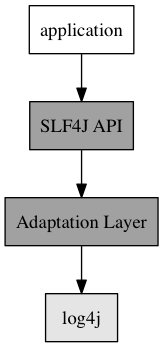
\includegraphics[width=0.5\linewidth, frame]{slf4j.png}
\caption{SLF4j Using log4j}
\label{fig:slf4jlog4j}
\end{figure}


In figure \ref{fig:slf4jlog4j} the application uses SLF4J to log. It has been bound to use log4j libraries through the adaptation layer. 

We can use the Java Logging API with SLF4J. A bit later we will swap the Java Logging API to log4j, and the code doesn't change at all.

First we will change our logging code to import the SLF4J Logger classes:
\begin{lstlisting}[language=Java]
import org.slf4j.Logger;
import org.slf4j.LoggerFactory;
\end{lstlisting}

Then we create a logger and use it to write our log messages:
\begin{lstlisting}[language=Java]
Logger logger = LoggerFactory.getLogger(this.getClass());
logger.error("Logging ERROR");
logger.warn("Logging WARN");
logger.info("Logging INFO");
logger.debug("Logging DEBUG");
\end{lstlisting}

See Appendix P on page \pageref{App:AppendixP} for the full source code for the  \texttt{ConfigLoggingEample.java} class.

In order to facilitate later swapping of the logging library, we will configure the logger in a configuration file. For Java Logging, the file is usually called \texttt{logging.properties}:
\begin{lstlisting}
handlers= java.util.logging.FileHandler, java.util.logging.ConsoleHandler
.level= FINEST

java.util.logging.FileHandler.pattern = simple.log
java.util.logging.FileHandler.limit = 50000
java.util.logging.FileHandler.count = 1
java.util.logging.FileHandler.formatter = java.util.logging.SimpleFormatter
java.util.logging.SimpleFormatter.format=%1$tb %1$td, %1$tY %1$tl:%1$tM:%1$tS %1$Tp %2$s %4$s: %5$s%n

java.util.logging.ConsoleHandler.level = FINEST
java.util.logging.ConsoleHandler.formatter = java.util.logging.SimpleFormatter
\end{lstlisting}

The source for \texttt{logging.properties} can be found in Appendix P on page \pageref{App:AppendixP}.

The first line specifies that we will use two handlers, one to log to a file and another to log to the console. The second block configures the file handler (lines 4-8). It specifies the name of the file, formatter and the format. We configure it to write to the \texttt{simple.log} file. The last block (lines 10-11)configures the console handler to use the \texttt{SimpleFormatter} also.

When we want to use the logging.properties (and Java Logging) with SLF4J, we need to trigger the runtime binding by adding a VM property to tell it where the file is when we run the program:
\begin{lstlisting}
java -cp ".:slf4j-jdk14-1.7.22.jar:slf4j-api-1.7.22.jar" -Djava.util.logging.config.file=./logging.properties org.familysearch.viitanenm.SimpleFormatterExample
\end{lstlisting}

We include the slf4j API library to the classpath (for our code) and also the binding library for Java Logging. Then we use the -Djava.util.logging.config.file Java Logging property to point to the configuration file.

The contents of the simple.log file with this configuration is:
\begin{lstlisting}
Dec 21, 2016 12:28:34 PM viitanenm.SimpleFormatterExample doIt SEVERE: Logging ERROR
Dec 21, 2016 12:28:35 PM viitanenm.SimpleFormatterExample doIt WARNING: Logging WARN
Dec 21, 2016 12:28:35 PM viitanenm.SimpleFormatterExample doIt INFO: Logging INFO
Dec 21, 2016 12:28:35 PM viitanenm.SimpleFormatterExample doIt FINE: Logging DEBUG
\end{lstlisting}

See how DEBUG translates into FINE level.

Java Logging has another formatter that we could use, XMLFormatter. We can swap to use it by changing the logging.properties file:

\begin{lstlisting}
java.util.logging.ConsoleHandler.formatter = java.util.logging.XMLFormatter
\end{lstlisting}

Now the output of the console handler changes to XML:
\begin{lstlisting}[language=XML]
<?xml version="1.0" encoding="UTF-8" standalone="no"?>
<!DOCTYPE log SYSTEM "logger.dtd">
<log>
<record>
  <date>2016-12-21T12:30:57</date>
  <millis>1482348657028</millis>
  <sequence>0</sequence>
  <logger>viitanenm.SimpleFormatterExample</logger>
  <level>SEVERE</level>
  <class>viitanenm.SimpleFormatterExample</class>
  <method>doIt</method>
  <thread>1</thread>
  <message>Logging ERROR</message>
</record>
<record>
  <date>2016-12-21T12:30:57</date>
  <millis>1482348657059</millis>
  <sequence>1</sequence>
  <logger>viitanenm.SimpleFormatterExample</logger>
  <level>WARNING</level>
  <class>viitanenm.SimpleFormatterExample</class>
  <method>doIt</method>
  <thread>1</thread>
  <message>Logging WARN</message>
</record>
<record>
  <date>2016-12-21T12:30:57</date>
  <millis>1482348657060</millis>
  <sequence>2</sequence>
  <logger>viitanenm.SimpleFormatterExample</logger>
  <level>INFO</level>
  <class>viitanenm.SimpleFormatterExample</class>
  <method>doIt</method>
  <thread>1</thread>
  <message>Logging INFO</message>
</record>
<record>
  <date>2016-12-21T12:30:57</date>
  <millis>1482348657060</millis>
  <sequence>3</sequence>
  <logger>viitanenm.SimpleFormatterExample</logger>
  <level>FINE</level>
  <class>viitanenm.SimpleFormatterExample</class>
  <method>doIt</method>
  <thread>1</thread>
  <message>Logging DEBUG</message>
</record>
\end{lstlisting}

There were no code changes made.

Log4j is another logging library that provides more functionality than Java Logging. The code itself doesn't change at all. We just configure bindings for slf4j. If we want to use log4j logging library, for example, instead of Java Logging, we just add those libraries in our classpath.

We create a log4j configuration file, \texttt{log4j2.prop\hyp{}erties}. 

The source for \texttt{log4j2.prop\hyp{}erties} can be found in Appendix P on page \pageref{App:AppendixP}.
\begin{lstlisting}
# log to the console
appender.console.type = Console
appender.console.name = STDOUT
appender.console.layout.type = PatternLayout
appender.console.layout.pattern = [%d{MM-dd-yy HH:mm:ss ZZZ}] [%p] [${hostName}] %m%n

# log to a file
appender.rolling.type = RollingFile
appender.rolling.name = RollingFile
appender.rolling.fileName = mylog.log
appender.rolling.filePattern = mylog-%d{yyyy-MM-dd-HH-mm-ss}-%i.log.gz
appender.rolling.layout.type = PatternLayout
appender.rolling.layout.pattern = [%d{MM-dd-yy HH:mm:ss ZZZ}] [%p] [${hostName}] %m%n
appender.rolling.policies.type = Policies
appender.rolling.policies.time.type = TimeBasedTriggeringPolicy
appender.rolling.policies.time.interval = 2
appender.rolling.policies.time.modulate = true
appender.rolling.policies.size.type = SizeBasedTriggeringPolicy
appender.rolling.policies.size.size=500B
appender.rolling.strategy.type = DefaultRolloverStrategy
appender.rolling.strategy.max = 5
 
logger.rolling.name = com.example.my.app
logger.rolling.level = debug
logger.rolling.additivity = true
logger.rolling.appenderRef.rolling.ref = RollingFile

#set the appender
rootLogger.level = info
rootLogger.appenderRef.stdout.ref = STDOUT
rootLogger.appenderRef.rolling.ref = RollingFile
\end{lstlisting}

Slf4j follows the \texttt{StringFormatter} syntax, but also adds some properties. In our pattern we first print the date, time, and timezone in brackets. Then we print the log level, also in brackets. Log4j provices access to the host name or IP address with the \texttt{hostName} property. We print that, and in the end our customized message from the code, followed by a new line.

Log4j automatically looks for a configuration file in the path, so we don't have to specify its location when we run the code.
\begin{lstlisting}
java -cp ".:slf4j-api-1.7.22.jar:log4j-api-2.7.jar:log4j-core-2.7.jar:log4j-slf4j-impl-2.7.jar"  org.familysearch.viitanenm.ConfigLoggingExample
\end{lstlisting}

We added the log4j libraries to the classpath. We have the slf4j api library, and three libraries from log4j; log4j api library, a core library, and a binding library (to bind slf4j and log4j). 

The output will be (with info level):
\begin{lstlisting}
[12-20-16 14:41:50 -07:00] [ERROR] [viitanenm.local] Logging ERROR
[12-20-16 14:41:50 -07:00] [WARN] [viitanenm.local] Logging WARN
[12-20-16 14:41:50 -07:00] [INFO] [viitanenm.local] Logging INFO
\end{lstlisting}

In the configuration file we defined a \texttt{RollingFile\hyp{}Appender} appender. It automatically archives the log files when they get to a specified size, or after specified time. In our example we configured it to roll when the file size is more than 500B. In practice that limit would be larger but we just want to test it.

After running the code several times, we can see the log file rolling:
\begin{lstlisting}
-rw-r--r--   87B Dec 20 14:41 mylog-2016-12-20-14-41-29-1.log.gz
-rw-r--r--   87B Dec 20 14:41 mylog-2016-12-20-14-41-33-1.log.gz
-rw-r--r--   87B Dec 20 14:41 mylog-2016-12-20-14-41-49-1.log.gz
-rw-r--r--  143B Dec 20 14:41 mylog.log
\end{lstlisting}


\phantomsection
\begin{thebibliography}{21}

\bibitem{spec}
James Gosling, Bill Joy, Guy Steele, Gilad Bracha, Alex Buckley. \textit{The Java® Language Specification.} The Java® Language Specification. Oracle America, Inc., 13 Feb. 2015. Web. 12 Dec. 2016. <\url{http://docs.oracle.com/javase/specs/jls/se8/html/index.html}>.

\qrcode[height=.5in]{http://docs.oracle.com/javase/specs/jls/se8/html/index.html}









\bibitem{gosling}
Gosling, James, Bill Joy, Guy Steele, Gilad Bracha, and Alex Buckley. \textit{The Java® Virtual Machine Specification.} The Java® Virtual Machine Specification. Oracle America, Inc, 28 Feb. 2013. Web. 12 Aug. 2014. <\url{https://docs.oracle.com/javase/specs/jvms/se7/html/}>.

\qrcode[height=.5in]{https://docs.oracle.com/javase/specs/jvms/se7/html/}


\bibitem{api}
\textit{Java Platform SE 7.} Java Platform SE 7. Oracle, n.d. Web. 12 Dec. 2014. <\url{http://docs.oracle.com/javase/7/docs/api/}>.

\qrcode[height=.5in]{http://docs.oracle.com/javase/7/docs/api/}

\bibitem{tutorial}
\textit{Trail: Learning the Java Language.} The Java™ Tutorials. Oracle, n.d. Web. 12 Dec. 2014. <\url{https://docs.oracle.com/javase/tutorial/java/index.html}>.

\qrcode[height=.5in]{https://docs.oracle.com/javase/tutorial/java/index.html}

\bibitem{nicholas}
Nicholas, Ethan. \textit{Understanding Weak References.} Understanding Weak References. Java.net, 4 May 2006. Web. 13 Dec. 2014. <\url{https://weblogs.java.net/Fblog/2006/05/04/understanding-weak-references}>.

\qrcode[height=.5in]{https://weblogs.java.net/Fblog/2006/05/04/understanding-weak-references}

\bibitem{reference}
\textit{Package java.lang.ref.} Java.lang.ref (Java Platform SE 7 ). Oracle, n.d. Web. 13 Dec. 2014. <\url{http://docs.oracle.com/javase/7/docs/api/java/lang/ref/package-summary.html}>.

\qrcode[height=.5in]{http://docs.oracle.com/javase/7/docs/api/java/lang/ref/package-summary.html}

\bibitem{garbagecollection}
\textit{Java Garbage Collection Basics.} Java Garbage Collection Basics. Oracle, n.d. Web. 13 Dec. 2014. <\url{http://www.oracle.com/webfolder/technetwork/tutorials/obe/java/gc01/index.html}>.

\qrcode[height=.5in]{http://www.oracle.com/webfolder/technetwork/tutorials/obe/java/gc01/index.html}

\bibitem{java7}
\textit{Java SE 7 Features and Enhancements.} Java SE 7 Features and Enhancements. Oracle, n.d. Web. 13 Dec. 2014. <\url{http://www.oracle.com/technetwork/java/javase/jdk7-relnotes-418459.html#jdk7changes}>.

\qrcode[height=.5in]{http://www.oracle.com/technetwork/java/javase/jdk7-relnotes-418459.html#jdk7changes}

\bibitem{gcergo}
\textit{Garbage Collector Ergonomics.} Garbage Collector Ergonomics. Oracle, n.d. Web. 13 Dec. 2014. <\url{http://docs.oracle.com/javase/7/docs/technotes/guides/vm/gc-ergonomics.html}>.

\qrcode[height=.5in]{http://docs.oracle.com/javase/7/docs/technotes/guides/vm/gc-ergonomics.html}

\bibitem{list}
\textit{Interface List<E>} Java™ Platform, Standard Edition 8
API Specification. Oracle, n.d. Web. 7 Dec. 2016. <\url{http://docs.oracle.com/javase/8/docs/api/java/util/List.html}>.

\qrcode[height=.5in]{http://docs.oracle.com/javase/8/docs/api/java/util/List.html}

\bibitem{map}
\textit{Interface Map<E>} Java™ Platform, Standard Edition 8
API Specification. Oracle, n.d. Web. 7 Dec. 2016. <\url{https://docs.oracle.com/javase/8/docs/api/java/util/Map.html}>.

\qrcode[height=.5in]{https://docs.oracle.com/javase/8/docs/api/java/util/Map.html}

\bibitem{set}
\textit{Interface Set<E>} Java™ Platform, Standard Edition 8
API Specification. Oracle, n.d. Web. 7 Dec. 2016. <\url{https://docs.oracle.com/javase/8/docs/api/java/util/Set.html}>.

\qrcode[height=.5in]{https://docs.oracle.com/javase/8/docs/api/java/util/Set.html}

\bibitem{error}
\textit{Class Error} Java™ Platform, Standard Edition 8
API Specification. Oracle, n.d. Web. 7 Dec. 2016. <\url{http://docs.oracle.com/javase/8/docs/api/java/lang/Error.html}>.

\qrcode[height=.5in]{http://docs.oracle.com/javase/8/docs/api/java/lang/Error.html}

\bibitem{exception}
\textit{Class Exception} Java™ Platform, Standard Edition 8
API Specification. Oracle, n.d. Web. 7 Dec. 2016. <\url{http://docs.oracle.com/javase/8/docs/api/java/lang/Exception.html}>.

\qrcode[height=.5in]{http://docs.oracle.com/javase/8/docs/api/java/lang/Exception.html}

\bibitem{runtimeexception}
\textit{Unchecked Exceptions — The Controversy} The Java™ Tutorials. Oracle, n.d. Web. 7 Dec. 2016. <\url{https://docs.oracle.com/javase/tutorial/essential/exceptions/runtime.html}>.

\qrcode[height=.5in]{https://docs.oracle.com/javase/tutorial/essential/exceptions/runtime.html}


\bibitem{codesmells}
\textit{Smells to Refactorings -- Quick Reference Guide} Industrial Logic, n.d. Web. 14 Dec. 2016. <\url{http://www.industriallogic.com/wp-content/uploads/2005/09/smellstorefactorings.pdf}>.

\qrcode[height=.5in]{http://www.industriallogic.com/wp-content/uploads/2005/09/smellstorefactorings.pdf}

\bibitem{referenceorvalue}
\textit{Does Java pass by reference or pass by value?} Java World, n.d. Web. 14 Dec. 2016. <\url{http://www.javaworld.com/article/2077424/learn-java/does-java-pass-by-reference-or-pass-\hyp{}by-value.html}>.

\qrcode[height=.5in]{http://www.javaworld.com/article/2077424/learn-java/does-java-pass-by-reference-or-pass-by-value.html}


\bibitem{slf4j}
\textit{Simple Logging Facade for Java (SLF4J)} slf4j.org, n.d. Web. 14 Dec. 2016. <\url{http://www.slf4j.org/}>.

\qrcode[height=.5in]{http://www.slf4j.org/}

\bibitem{simplelogger}
\textit{Class SimpleLogger} SLF4J 1.7.22 API, n.d. Web. 14 Dec. 2016. <\url{http://www.slf4j.org/api/org/slf4j/impl/SimpleLogger.html}>.

\qrcode[height=.5in]{http://www.slf4j.org/api/org/slf4j/impl/SimpleLogger.html}

\bibitem{slf4jmanual}
\textit{SLF4J user manual} slf4j.org, n.d. Web. 14 Dec. 2016. <\url{http://www.slf4j.org/manual.html}>.

\qrcode[height=.5in]{http://www.slf4j.org/manual.html}

\bibitem{level}
\textit{Class Level} Java™ Platform, Standard Edition 8
API Specification. Oracle, n.d. Web. 14 Dec. 2016. <\url{https://docs.oracle.com/javase/8/docs/api/java/util/logging/Level.html}>.

\qrcode[height=.5in]{https://docs.oracle.com/javase/8/docs/api/java/util/logging/Level.html}
\end{thebibliography}

\onecolumn
\phantomsection
\section*{Appendix} % The \section*{} command stops section numbering

\addcontentsline{toc}{section}{Appendix} % Adds this section to the table of contents

\appendix
\subsection*{Appendix A -- Garbage Collection} \label{App:AppendixA}
\addcontentsline{toc}{subsection}{Appendix A -- Garbage Collection} % Adds this section to the table of contents

\subsubsection*{org.familysearch.viitanenm.gc.GarbageCollectionExample.java}
\noindent\begin{minipage}{.6in}
  \qrcode[height=.5in]{https://raw.githubusercontent.com/mviitanen/ati-java-apprentice/master/code/1-1-garbage-collection/src/org/familysearch/viitanenm/gc/GarbageCollectionExample.java}
\end{minipage}
%  \hspace{0.3cm}% adjust for horizontal spacing
\begin{minipage}{6in}
  \url{https://raw.githubusercontent.com/mviitanen/ati-java-apprentice/master/code/1-1-garbage-collection/src/org/familysearch/viitanenm/gc/GarbageCollectionExample.java}
\end{minipage}

\vspace{1em}
\subsubsection*{org.familysearch.viitanenm.gc.DataSizePrinter.java}
\noindent\begin{minipage}{.6in}
      \qrcode[height=.5in]{https://raw.githubusercontent.com/mviitanen/ati-java-apprentice/master/code/1-1-garbage-collection/src/org/familysearch/viitanenm/gc/DataSizePrinter.java}
    \end{minipage}
 % \hspace{0.3cm}% adjust for horizontal spacing
    \begin{minipage}{6in}    
      \url{https://raw.githubusercontent.com/mviitanen/ati-java-apprentice/master/code/1-1-garbage-collection/src/org/familysearch/viitanenm/gc/DataSizePrinter.java}
    \end{minipage}
\subsection*{Appendix B -- Strings} \label{App:AppendixB}
\addcontentsline{toc}{subsection}{Appendix B -- Strings} % Adds this section to the table of contents

\subsubsection*{org.familysearch.viitanenm.StringExample.java}
\noindent
\begin{minipage}{.6in}
  \qrcode[height=.5in]{https://raw.githubusercontent.com/mviitanen/ati-java-apprentice/master/code/1-2-internal-string/src/org/familysearch/viitanenm/StringExample.java}
\end{minipage}
\begin{minipage}{6in}
  \url{https://raw.githubusercontent.com/mviitanen/ati-java-apprentice/master/code/1-2-internal-string/src/org/familysearch/viitanenm/StringExample.java}
\end{minipage}

\subsection*{Appendix C -- List of Strings} \label{App:AppendixC}
\addcontentsline{toc}{subsection}{Appendix C -- List of Strings} % Adds this section to the table of contents

\subsubsection*{org.familysearch.viitanenm.ListOfStringsExample.java}
\noindent
\begin{minipage}{.6in}
  \qrcode[height=.5in]{https://raw.githubusercontent.com/mviitanen/ati-java-apprentice/master/code/1-3-list-of-strings/src/org/familysearch/viitanenm/ListOfStringsExample.java}
\end{minipage}
\begin{minipage}{6in}
  \url{https://raw.githubusercontent.com/mviitanen/ati-java-apprentice/master/code/1-3-list-of-strings/src/org/familysearch/viitanenm/ListOfStringsExample.java}
\end{minipage}
\subsection*{Appendix D -- StringBuffer and StringBuilder} \label{App:AppendixD}
\addcontentsline{toc}{subsection}{Appendix D} % Adds this section to the table of contents
\qrcode[height=.5in]{http://google.com}
\begin{lstlisting}[language=Java]
package org.familysearch.viitanenm;

import java.io.BufferedWriter;
import java.io.FileOutputStream;
import java.io.IOException;
import java.io.OutputStreamWriter;
import java.io.Writer;
import java.text.DecimalFormat;
import java.text.NumberFormat;

public class Main {
  private static final String SHORT_STR = "a";
  private static final String KINDA_SHORT_STR = "aaaaa";
  private static final String MEDIUM_STR = "aaaaaaaaaa";
  private static final String KINDA_LONG_STR = "aaaaaaaaaaaaaaaaaaaaaaaaa";
  private static final String LONG_STR = "aaaaaaaaaaaaaaaaaaaaaaaaaaaaaaaaaaaaaaaaaaaaaaaaaa";
  private static final String[] strs = {SHORT_STR, KINDA_SHORT_STR, MEDIUM_STR, KINDA_LONG_STR, LONG_STR};
  private static long start;
  private static long end;
  private static long delta;
  private static NumberFormat fmt = new DecimalFormat("#0.000000000");

  public static void main(String[] args) {
    Writer builderWriter = null;
    Writer bufferWriter = null;
    try {
      builderWriter = new BufferedWriter(new OutputStreamWriter(
          new FileOutputStream("builder.txt"), "utf-8"));
      bufferWriter = new BufferedWriter(new OutputStreamWriter(
          new FileOutputStream("buffer.txt"), "utf-8"));
      for (String str : strs) {
        long bufferStrTotal = 0;
        long builderStrTotal = 0;
        int counter = 0;
        for (int i = 1000000; i <= 10000000; i += 1000000) {
          doItBuffer(str, i, bufferWriter);
          bufferStrTotal += delta;
          doItBuilder(str, i, builderWriter);
          builderStrTotal += delta;
          counter++;
        }
        System.out.println("Buffer average by string length ("+str.length()+"):" + (bufferStrTotal/counter));
        System.out.println("Builder average by string length ("+str.length()+"):" + (builderStrTotal/counter));
      }

      for (int i = 1000000; i <= 10000000; i += 1000000) {
        long bufferStrTotal = 0;
        long builderStrTotal = 0;
        int counter = 0;
        for (String str : strs) {
          doItBuffer(str, i, bufferWriter);
          bufferStrTotal += delta;
          doItBuilder(str, i, builderWriter);
          builderStrTotal += delta;
          counter++;
        }
        System.out.println("Buffer average by additions ("+i+"):" + (bufferStrTotal/counter));
        System.out.println("Builder average by additions ("+i+"):" + (builderStrTotal/counter));
      }

    } catch (Exception e) {
      e.printStackTrace();
    } finally {
      if (builderWriter != null) {
        try {
          builderWriter.close();
        } catch (IOException e) {
          e.printStackTrace();
        }
      }
      if (bufferWriter != null) {
        try {
          bufferWriter.close();
        } catch (IOException e) {
          e.printStackTrace();
        }
      }
    }
  }

  private static void doItBuffer(String str, int counter, Writer writer) throws IOException {
    String msg = "";
    StringBuffer buffer = new StringBuffer();
    try {
      start = System.currentTimeMillis();
      for (int i = 0; i < counter; i++) {
        buffer.append(str);
      }
      end = System.currentTimeMillis();
      delta = end - start;
    } catch (Throwable e) {
      delta = 0;
    } finally {

      String fullMsg = str.length() + "\t" + counter + "\t" + delta + "\t" + fmt.format(((double) delta / (double) counter)) + "\tbuffer\t" + msg;
      writer.append(fullMsg + "\n");
      //System.out.println(fullMsg);
    }
  }

  private static void doItBuilder(String str, int counter, Writer writer) throws IOException {
    String msg = "";
    StringBuilder builder = new StringBuilder();
    try {
      start = System.currentTimeMillis();
      for (int i = 0; i < counter; i++) {
        builder.append(str);
      }
      end = System.currentTimeMillis();
      delta = end - start;
    } catch (Throwable e) {
      msg = "E!";
      delta = 0;
    } finally {

      String fullMsg = str.length() + "\t" + counter + "\t" + delta + "\t" + fmt.format(((double) delta / (double) counter)) + "\tbuilder\t" + msg;
      writer.append(fullMsg + "\n");
      //System.out.println(fullMsg);
    }
  }
}
\end{lstlisting}
\subsection*{Appendix E -- StringBuilder Concurrency} \label{App:AppendixE}
\addcontentsline{toc}{subsection}{Appendix E -- StringBuilder Concurrency} % Adds this section to the table of contents

\subsubsection*{org.familysearch.viitanenm.StringBuilderStringBufferConcurrencyExample.java}
\noindent
\begin{minipage}{.6in}
  \qrcode[height=.5in]{https://raw.githubusercontent.com/mviitanen/ati-java-apprentice/master/code/1-4-b-string-buffer-string-builder-concurrency/src/org/familysearch/viitanenm/StringBuilderStringBufferConcurrencyExample.java}
\end{minipage}
\begin{minipage}{6in}
  \url{https://raw.githubusercontent.com/mviitanen/ati-java-apprentice/master/code/1-4-b-string-buffer-string-builder-concurrency/src/org/familysearch/viitanenm/StringBuilderStringBufferConcurrencyExample.java}
\end{minipage}

\subsubsection*{builder-hex.txt}
\noindent
\begin{minipage}{.6in}
  \qrcode[height=.5in]{https://raw.githubusercontent.com/mviitanen/ati-java-apprentice/master/code/1-4-b-string-buffer-string-builder-concurrency/builder-hex.txt}
\end{minipage}
\begin{minipage}{6in}
  \url{https://raw.githubusercontent.com/mviitanen/ati-java-apprentice/master/code/1-4-b-string-buffer-string-builder-concurrency/builder-hex.txt}
\end{minipage}


\subsection*{Appendix F -- Sorting In Memory} \label{App:AppendixF}
\addcontentsline{toc}{subsection}{Appendix F} % Adds this section to the table of contents
\qrcode[height=.5in]{http://google.com}
\begin{lstlisting}[language=Java]
package org.familysearch.viitanenm;

import java.io.BufferedWriter;
import java.io.FileNotFoundException;
import java.io.FileOutputStream;
import java.io.IOException;
import java.io.OutputStreamWriter;
import java.io.UnsupportedEncodingException;
import java.io.Writer;
import java.nio.file.Files;
import java.nio.file.Path;
import java.nio.file.Paths;
import java.util.Comparator;
import java.util.List;

public class MainInMemory {
  public static void main(String[] args) {
    try {
      new MainInMemory().doIt();
    } catch (IOException e) {
      e.printStackTrace();
    }
  }

  private void doIt() throws IOException {
    sortInMemory();
  }

  private void sortInMemory() throws IOException {
    Path in = Paths.get(".", "lorem.txt");
    List<String> lines = Files.readAllLines(in);
    long start = System.currentTimeMillis();
    lines.sort(new Comparator<String>() {
      @Override
      public int compare(String left, String right) {
        return left.compareTo(right);
      }
    });
    long end = System.currentTimeMillis();
    System.out.println("In memory sort (" + lines.size() + " lines) took " + (end - start) + " ms");
    Writer writer = null;
    try {
      writer = new BufferedWriter(new OutputStreamWriter(
          new FileOutputStream("out-in-memory.txt"), "utf-8"));
      for (String line : lines) {
        writer.write(line + '\n');
      }

    } catch (UnsupportedEncodingException e) {
      e.printStackTrace();
    } catch (FileNotFoundException e) {
      e.printStackTrace();
    } catch (IOException e) {
      e.printStackTrace();
    } finally {
      if (writer != null) {
        try {
          writer.close();
        } catch (IOException e) {
          e.printStackTrace();
        }
      }
    }
  }
}
\end{lstlisting}
\subsection*{Appendix G -- Sorting} \label{App:AppendixG}
\addcontentsline{toc}{subsection}{Appendix G -- Sorting} % Adds this section to the table of contents

\subsubsection*{org.familysearch.viitanenm.SortInMemoryExample.java}
\noindent
\begin{minipage}{.6in}
  \qrcode[height=.5in]{https://raw.githubusercontent.com/mviitanen/ati-java-apprentice/master/code/1-6-7-sorting/src/org/familysearch/viitanenm/SortInMemoryExample.java}
\end{minipage}
\begin{minipage}{6in}
  \url{https://raw.githubusercontent.com/mviitanen/ati-java-apprentice/master/code/1-6-7-sorting/src/org/familysearch/viitanenm/SortInMemoryExample.java}
\end{minipage}

\vspace{1em}
\subsubsection*{org.familysearch.viitanenm.SortInFileExample.java}
\noindent
\begin{minipage}{.6in}
  \qrcode[height=.5in]{https://raw.githubusercontent.com/mviitanen/ati-java-apprentice/master/code/1-6-7-sorting/src/org/familysearch/viitanenm/SortInFileExample.java}
\end{minipage}
\begin{minipage}{6in}
  \url{https://raw.githubusercontent.com/mviitanen/ati-java-apprentice/master/code/1-6-7-sorting/src/org/familysearch/viitanenm/SortInFileExample.java}
\end{minipage}

\vspace{1em}
\subsubsection*{org.familysearch.viitanenm.ReverseSortInMemoryExample.java}
\noindent
\begin{minipage}{.6in}
  \qrcode[height=.5in]{https://raw.githubusercontent.com/mviitanen/ati-java-apprentice/master/code/1-6-7-sorting/src/org/familysearch/viitanenm/ReverseSortInMemoryExample.java}
\end{minipage}
\begin{minipage}{6in}
  \url{https://raw.githubusercontent.com/mviitanen/ati-java-apprentice/master/code/1-6-7-sorting/src/org/familysearch/viitanenm/ReverseSortInMemoryExample.java}
\end{minipage}

\vspace{1em}
\subsubsection*{org.familysearch.viitanenm.SortReverseInFileExample.java}
\noindent
\begin{minipage}{.6in}
  \qrcode[height=.5in]{https://raw.githubusercontent.com/mviitanen/ati-java-apprentice/master/code/1-6-7-sorting/src/org/familysearch/viitanenm/SortReverseInFileExample.java}
\end{minipage}
\begin{minipage}{6in}
  \url{https://raw.githubusercontent.com/mviitanen/ati-java-apprentice/master/code/1-6-7-sorting/src/org/familysearch/viitanenm/SortReverseInFileExample.java}
\end{minipage}
\subsection*{Appendix H -- Exception} \label{App:AppendixH}
\addcontentsline{toc}{subsection}{Appendix H} % Adds this section to the table of contents
\qrcode[height=.5in]{http://google.com}
\subsubsection{A Specialized Exception}
\begin{lstlisting}[language=Java]
package org.familysearch.viitanenm;

/**
 * A specialized Exception that also captures the error code
 */
public class MyException extends Exception {

  private int errorCode;

  public MyException(int errorCode) {
    this.errorCode = errorCode;
  }

  public MyException(Throwable cause, int errorCode) {
    super(cause);
    this.errorCode = errorCode;
  }

  public MyException(String message, int errorCode) {
    super(message);
    this.errorCode = errorCode;
  }

  public MyException(String message, Throwable cause, int errorCode) {
    super(message, cause);
    this.errorCode = errorCode;
  }

  public int getErrorCode() {
    return errorCode;
  }

  public void setErrorCode(int errorCode) {
    this.errorCode = errorCode;
  }
}
\end{lstlisting}

\subsubsection{Throwing and Catching an Exception}\label{App:AppendixHThrowCatch}
\begin{lstlisting}[language=Java]
package org.familysearch.viitanenm;

public class ExceptionExample {

  private boolean someConditionIsTrue = true;

  public static void main(String[] args) {
    new ExceptionExample().doIt();
  }

  private void doIt() {
    catchCheckedException();
    System.out.println();
    catchThrowError();
    System.out.println();
    catchCustomException();
    System.out.println();
    catchUncheckedException();
  }

  /**
   * Demonstrates throwing an unchecked exception.
   * <p/>
   * Notice how there is no <code>throws</code> statement in the method signature
   */
  private void throwUncheckedException() {
    if (someConditionIsTrue) {
      throw new IllegalArgumentException("This is my error message");
    } else {
      System.out.println("Don't throw it, then...");
    }
  }

  private void catchUncheckedException() {
    System.out.println("About to call a method that throws an unchecked exception, handled");

    try {
      throwUncheckedException();
    } catch (RuntimeException e) {
      System.out.println("Exception caught: " + e.getMessage());
    } finally {
      System.out.println("Finally");
    }
    System.out.println("Done calling a method that throws an unchecked exception, handled");
    System.out.println("About to call a method that throws an unchecked exception, not handled");
    throwUncheckedException();
    System.out.println("Done calling a method that throws an unchecked exception, not handled");
  }

  private void throwCheckedException() throws IllegalArgumentException {
    if (someConditionIsTrue) {
      throw new IllegalArgumentException("This is my custom exception message");
    } else {
      System.out.println("Don't throw it, then...");
    }
  }

  private void catchCheckedException() {
    System.out.println("About to call a method that throws a checked exception, handled");

    try {
      throwCheckedException();
    } catch (IllegalArgumentException e) {
      System.out.println("Exception caught: " + e.getMessage());
    } finally {
      System.out.println("Finally");
    }
    System.out.println("Done calling a method that throws a checked exception, handled");
  }

  private void throwError() {
    throw new UnknownError("This is my unknown error");
  }

  private void catchThrowError() {
    System.out.println("About to call a method that throws an error, handled");

    try {
      throwError();
    } catch (UnknownError e) {
      System.out.println("Error caught: " + e.getMessage());
    } finally {
      System.out.println("Finally");
    }
    System.out.println("Done calling a method that throws an error, handled");
  }

  private void throwCustomException() throws MyException {
    if (someConditionIsTrue) {
      throw new MyException("This is my custom exception message", 404);
    } else {
      System.out.println("Don't throw it, then...");
    }
  }

  private void catchCustomException() {
    System.out.println("About to call a method that throws a custom exception, handled");

    try {
      throwCustomException();
    } catch (MyException e) {
      System.out.println("Exception caught: " + e.getMessage());
    } finally {
      System.out.println("Finally");
    }
    System.out.println("Done calling a method that throws a custom exception, handled");
  }
}

\end{lstlisting}


%----------------------------------------------------------------------------------------

\end{document}